
%% DC Circuit Questions used on the
%% NYSED Physics Regents Examination
%%--------------------------------------------------

%% this section contains 185 problems

%% NOTE: replace ammeter with node[anchor=center] {$A$};

%% TODO: \draw (0,0) to node[currarrow] {} (1,0);

%% Section June2015
%%--------------------
\element{nysed}{
\begin{question}{June2015-Q13}
    A radio operating at \SI{3.0}{\volt} and a constant temperature draws a current of \SI{1.8e-4}{\ampere}.
    What is the resistance of the radio circuit?
    \begin{multicols}{2}
    \begin{choices}
      \correctchoice{\SI{1.7e4}{\ohm}}
        \wrongchoice{\SI{3.0e1}{\ohm}}
        \wrongchoice{\SI{5.4e-4}{\ohm}}
        \wrongchoice{\SI{6.0e-5}{\ohm}}
    \end{choices}
    \end{multicols}
\end{question}
}

\element{nysed}{
\begin{question}{June2015-Q17}
    During a laboratory experiment,
        a student finds that at \SI{20}{\degreeCelsius},
        a \SI{6.0}{\meter} length of copper wire has a resistance of \SI{1.3}{\ohm}. 
    The cross-sectional area of this wire is:
    \begin{multicols}{2}
    \begin{choices}
        %% NOTE: \rho_{Cu} = 1.68e-8 \ohm\meter
      \correctchoice{\SI{7.9e-8}{\meter\squared}}
        \wrongchoice{\SI{1.1e-7}{\meter\squared}}
        \wrongchoice{\SI{4.6e0}{\meter\squared}}
        \wrongchoice{\SI{1.3e7}{\meter\squared}}
    \end{choices}
    \end{multicols}
\end{question}
}

\element{nysed}{
\begin{question}{June2015-Q18}
    A net charge of \SI{5.0}{\coulomb} passes a point on a conductor in \SI{0.050}{\second}. 
    The average current is:
    \begin{multicols}{2}
    \begin{choices}
        \wrongchoice{\SI{8.0e-8}{\ampere}}
        \wrongchoice{\SI{1.0e-2}{\ampere}}
        \wrongchoice{\SI{2.5e-1}{\ampere}}
      \correctchoice{\SI{1.0e2}{\ampere}}
    \end{choices}
    \end{multicols}
\end{question}
}

\element{nysed}{
\begin{question}{June2015-Q19}
    If several resistors are connected in series in an electric circuit,
        the potential difference across each resistor:
    \begin{choices}
      \correctchoice{varies directly with its resistance.}
        \wrongchoice{varies inversely with its resistance.}
        \wrongchoice{varies inversely with the square of its resistance.}
        \wrongchoice{is independent of its resistance.}
    \end{choices}
\end{question}
}


%% Section June2014
%%--------------------
\element{nysed}{
\begin{question}{June2014-Q14}
    What is the resistance of a \SI{20.0}{\meter} long tungsten rod with a cross sectional area of \SI{1.00e-4}{\meter\squared} at \SI{20}{\degreeCelsius}
    \begin{multicols}{2}
    \begin{choices}
        \wrongchoice{\SI{2.8e-5}{\ohm}}
      \correctchoice{\SI{1.12e-2}{\ohm}}
        \wrongchoice{\SI{89.3}{\ohm}}
        \wrongchoice{\SI{112}{\ohm}}
    \end{choices}
    \end{multicols}
\end{question}
}

\element{nysed}{
\begin{question}{June2014-Q22}
    An MP3 player draws a current of \SI{0.120}{\ampere} from a \SI{3.00}{\volt} battery.
    What is the total charge that passes through the player in \SI{900}{second}?
    \begin{multicols}{2}
    \begin{choices}
      \correctchoice{\SI{108}{\coulomb}}
        \wrongchoice{\SI{324}{\coulomb}}
        \wrongchoice{\SI{5.40}{\coulomb}}
        \wrongchoice{\SI{1.80}{\coulomb}}
    \end{choices}
    \end{multicols}
\end{question}
}

\element{nysed}{
\begin{question}{June2014-Q40}
    The total amount of electrical energy used by a \SI{315}{\watt} television during \SI{30.0}{\minute} of operation is:
    \begin{multicols}{2}
    \begin{choices}
      \correctchoice{\SI{5.67e5}{\joule}}
        \wrongchoice{\SI{9.45e3}{\joule}}
        \wrongchoice{\SI{1.05e1}{\joule}}
        \wrongchoice{\SI{1.75e-1}{\joule}}
    \end{choices}
    \end{multicols}
\end{question}
}


%% Section June2013
%%--------------------
\element{nysed}{
\begin{question}{June2013-Q30}
    Moving \SI{4.0}{\coulomb} of charge through a circuit requires \SI{48}{\joule} of electric energy.
    What is the potential difference across this circuit?
    \begin{multicols}{2}
    \begin{choices}
        \wrongchoice{\SI{190}{\volt}}
        \wrongchoice{\SI{48}{\volt}}
      \correctchoice{\SI{12}{\volt}}
        \wrongchoice{\SI{4.0}{\volt}}
    \end{choices}
    \end{multicols}
\end{question}
}

\element{nysed}{
\begin{question}{June2013-Q31}
    The diagram below shows currents in a segment of an electric circuit.
    \begin{center}
    \ctikzset{bipoles/length=0.75cm}
    \begin{circuitikz}[scale=0.8]
        %% NOTE: this is a good reference
        \draw[thick] (-3,0) to [short,i^>=\SI{5}{\ampere}] (0,0)
                            to [short,i^>=\SI{3}{\ampere}] (3,0);
        \draw[thick] (0,2)  to [short,i^>=\SI{7}{\ampere}] (0,0)
                            to [ammeter] (0,-2);
    \end{circuitikz}
    \end{center}
    What is the reading of the ammeter?
    \begin{multicols}{2}
    \begin{choices}
        \wrongchoice{\SI{1}{\ampere}}
        \wrongchoice{\SI{5}{\ampere}}
      \correctchoice{\SI{9}{\ampere}}
        \wrongchoice{\SI{15}{\ampere}}
    \end{choices}
    \end{multicols}
\end{question}
}

\element{nysed}{
\begin{question}{June2013-Q32}
    An electric dryer consumes \SI{6.0e6}{\joule} of electrical energy when operating at \SI{220}{\volt} for \SI{1.8e3}{\second}.
    During operation, the dryer draws a current of:
    \begin{multicols}{2}
    \begin{choices}
        \wrongchoice{\SI{10}{\ampere}}
      \correctchoice{\SI{15}{\ampere}}
        \wrongchoice{\SI{9.0e2}{\ampere}}
        \wrongchoice{\SI{3.3e3}{\ampere}}
    \end{choices}
    \end{multicols}
\end{question}
}

\element{nysed}{
\begin{question}{June2013-Q42}
    The current in a wire is \SI{4.0}{\ampere}.
    The time required for \num{2.5e19} electrons to pass a certain point in the wire is:
    \begin{multicols}{2}
    \begin{choices}
      \correctchoice{\SI{1.0}{\second}}
        \wrongchoice{\SI{0.25}{\second}}
        \wrongchoice{\SI{0.50}{\second}}
        \wrongchoice{\SI{4.0}{\second}}
    \end{choices}
    \end{multicols}
\end{question}
}


%% Section June2012
%%--------------------
\element{nysed}{
\begin{question}{June2012-Q15}
    Which change decreases the resistance of a piece of copper wire?
    \begin{choices}
        \wrongchoice{increasing the wire's length}
        \wrongchoice{increasing the wire's resistivity}
      \correctchoice{decreasing the wire's temperature}
        \wrongchoice{decreasing the wire's diameter}
    \end{choices}
\end{question}
}

\element{nysed}{
\begin{question}{June2012-Q20}
    The resistance of a circuit remains constant.
    Which graph best represents the relationship between the current in the circuit and the potential difference provided by the battery?
    \begin{multicols}{2}
    \begin{choices}
        \AMCboxDimensions{down=-1.5em}
        \correctchoice{
            \begin{tikzpicture}
                \begin{axis}[
                    axis y line=left,
                    axis x line=bottom,
                    axis line style={->},
                    ylabel={current},
                    ytick=\empty,
                    xlabel={potential},
                    xtick=\empty,
                    xmin=0,xmax=11,
                    ymin=0,ymax=11,
                    width=\columnwidth,
                    very thin,
                ]
                \addplot[line width=1pt,domain=0:10]{x};
                \end{axis}
            \end{tikzpicture}
        }
        \wrongchoice{
            \begin{tikzpicture}
                \begin{axis}[
                    axis y line=left,
                    axis x line=bottom,
                    axis line style={->},
                    ylabel={current},
                    ytick=\empty,
                    xlabel={potential},
                    xtick=\empty,
                    xmin=0,xmax=11,
                    ymin=0,ymax=11,
                    width=\columnwidth,
                    very thin,
                ]
                \addplot[line width=1pt,domain=0:10]{0.1*x^2};
                \end{axis}
            \end{tikzpicture}
        }
        \wrongchoice{
            \begin{tikzpicture}
                \begin{axis}[
                    axis y line=left,
                    axis x line=bottom,
                    axis line style={->},
                    ylabel={current},
                    ytick=\empty,
                    xlabel={potential},
                    xtick=\empty,
                    xmin=0,xmax=11,
                    ymin=0,ymax=11,
                    width=\columnwidth,
                    very thin,
                ]
                \addplot[line width=1pt,domain=0:10]{10/x};
                \end{axis}
            \end{tikzpicture}
        }
        \wrongchoice{
            \begin{tikzpicture}
                \begin{axis}[
                    axis y line=left,
                    axis x line=bottom,
                    axis line style={->},
                    ylabel={current},
                    ytick=\empty,
                    xlabel={potential},
                    xtick=\empty,
                    xmin=0,xmax=11,
                    ymin=0,ymax=11,
                    width=\columnwidth,
                    very thin,
                ]
                \addplot[line width=1pt,domain=0:10]{8};
                \end{axis}
            \end{tikzpicture}
        }
    \end{choices}
    \end{multicols}
\end{question}
}

\element{nysed}{
\begin{question}{June2012-Q25}
    A \SI{3.0}{\ohm} resistor and a \SI{6.0}{\ohm} resistor are connected in parallel across a \SI{9}{\volt} battery.
    Which statement best compares the potential difference across each resistor?
    \begin{choices}
      \correctchoice{The potential difference across the \SI{6.0}{\ohm} resistor is the same as the potential difference across the \SI{3.0}{\ohm} resistor}
        \wrongchoice{The potential difference across the \SI{6.0}{\ohm} resistor is twice as great as the potential difference across the \SI{3.0}{\ohm} resistor}
        \wrongchoice{The potential difference across the \SI{6.0}{\ohm} resistor is half as great as the potential difference across the \SI{3.0}{\ohm} resistor}
        \wrongchoice{The potential difference across the \SI{6.0}{\ohm} resistor is four times as great as the potential difference across the \SI{3.0}{\ohm} resistor}
    \end{choices}
\end{question}
}

\element{nysed}{
\begin{question}{June2012-Q26}
    A \SI{3.6}{\volt} battery is used to operate a cell phone for \SI{5.0}{\minute}.
    If the cell phone dissipates \SI{0.064}{\watt} of power during its operation, the current that passes through the phone is:
    \begin{multicols}{2}
    \begin{choices}
      \correctchoice{\SI{0.018}{\ampere}}
        \wrongchoice{\SI{5.3}{\ampere}}
        \wrongchoice{\SI{19}{\ampere}}
        \wrongchoice{\SI{56}{\ampere}}
    \end{choices}
    \end{multicols}
\end{question}
}

\element{nysed}{
\begin{question}{June2012-Q41}
    What is the current in a wire if \num{3.4e19} electrons pass by a point in this wire every \SI{60}{\second}?
    \begin{multicols}{2}
    \begin{choices}
        \wrongchoice{\SI{1.8e-18}{\ampere}}
        \wrongchoice{\SI{3.1e-11}{\ampere}}
      \correctchoice{\SI{9.1e-2}{\ampere}}
        \wrongchoice{\SI{11}{\ampere}}
    \end{choices}
    \end{multicols}
\end{question}
}

\element{nysed}{
\begin{question}{June2012-Q43}
    To increase the brightness of a desk lamp, a student replaces a \SI{50}{\watt} incandescent lightbulb with a \SI{100}{\watt} incandescent lightbulb.
    Compared to the \SI{50}{\watt} lightbulb, the \SI{100}{\watt} lightbulb has:
    \begin{choices}
      \correctchoice{less resistance and draws more current.}
        \wrongchoice{less resistance and draws less current.}
        \wrongchoice{more resistance and draws more current.}
        \wrongchoice{more resistance and draws less current.}
    \end{choices}
\end{question}
}


%% Section June2011
%%--------------------
\element{nysed}{
\begin{question}{June2011-Q20}
    What is the current through a wire if \SI{240}{\coulomb} of charge pass through the wire in \SI{2.0}{\minute}?
    \begin{multicols}{2}
    \begin{choices}
        \wrongchoice{\SI{120}{\ampere}}
      \correctchoice{\SI{2.0}{\ampere}}
        \wrongchoice{\SI{0.50}{\ampere}}
        \wrongchoice{\SI{0.0083}{\ampere}}
    \end{choices}
    \end{multicols}
\end{question}
}

\element{nysed}{
\begin{question}{June2011-Q21}
    An electric circuit consists of a variable resistor connected to a source of constant potential difference.
    If the resistance of the resistor is doubled,
        the current through the resistor is:
    \begin{multicols}{2}
    \begin{choices}
      \correctchoice{halved}
        \wrongchoice{doubled}
        \wrongchoice{quartered}
        \wrongchoice{quadrupled}
    \end{choices}
    \end{multicols}
\end{question}
}

\element{nysed}{
\begin{question}{June2011-Q22}
    Circuit $A$ has four \SI{3.0}{\ohm} resistors connected in series with a \SI{24}{\volt} battery,
        and circuit $B$ has two \SI{3.0}{\ohm} resistors connected in series with a \SI{24}{\volt} battery.
    Compared to the total potential drop across circuit $A$,
        the total potential drop across circuit $B$ is:
    \begin{choices}
        \wrongchoice{one-half as great}
        \wrongchoice{twice as great}
      \correctchoice{the same}
        \wrongchoice{four times as great}
    \end{choices}
\end{question}
}

\element{nysed}{
\begin{question}{June2011-Q23}
    How much total energy is dissipated in \SI{10}{\second} in a \SI{4.0}{\ohm} resistor with a current of \SI{0.50}{\ampere}?
    \begin{multicols}{2}
    \begin{choices}
        \wrongchoice{\SI{2.5}{\joule}}
        \wrongchoice{\SI{5.0}{\joule}}
      \correctchoice{\SI{10}{\joule}}
        \wrongchoice{\SI{20}{\joule}}
    \end{choices}
    \end{multicols}
\end{question}
}

\element{nysed}{
\begin{question}{June2011-Q44}
    The diagram below represents a circuit consisting of two resistors connected to a source of potential difference.
    \begin{center}
    \ctikzset{bipoles/length=0.75cm}
    \begin{circuitikz}[xscale=1.25]
        \draw (0,0) to [battery,l=$\SI{120}{\volt}$] (0,2)
                    to [R,l=$\SI{10}{\ohm}$] (2,2)
                    to [R,l=$\SI{20}{\ohm}$] (2,0)
                    to (0,0);
    \end{circuitikz}
    \end{center}
    What is the current through the \SI{20}{\ohm} resistor?
    \begin{multicols}{2}
    \begin{choices}
        \wrongchoice{\SI{0.25}{\ampere}}
        \wrongchoice{\SI{6.0}{\ampere}}
        \wrongchoice{\SI{12}{\ampere}}
      \correctchoice{\SI{4.0}{\ampere}}
    \end{choices}
    \end{multicols}
\end{question}
}


%% Section June2010
%%--------------------
\element{nysed}{
\begin{question}{June2010-Q18}
    An electric heater operating at \SI{120}{\volt} draws \SI{8.00}{\ampere} of current through its \SI{15.0}{\ohm} of resistance.
    The total amount of heat energy produces by the heater in \SI{60}{\second} is by the box?
    \begin{multicols}{2}
    \begin{choices}
        \wrongchoice{\SI{7.20e3}{\joule}}
      \correctchoice{\SI{5.76e4}{\joule}}
        \wrongchoice{\SI{8.64e4}{\joule}}
        \wrongchoice{\SI{6.91e6}{\joule}}
    \end{choices}
    \end{multicols}
\end{question}
}

\element{nysed}{
\begin{question}{June2010-Q20}
    A charge of \SI{30}{\coulomb} passes through a \SI{24}{\ohm} resistor in \SI{6.0}{\second}.
    What is the current through the resistor?
    \begin{multicols}{2}
    \begin{choices}
        \wrongchoice{\SI{1.3}{\ampere}}
      \correctchoice{\SI{5.0}{\ampere}}
        \wrongchoice{\SI{7.5}{\ampere}}
        \wrongchoice{\SI{4.0}{\ampere}}
    \end{choices}
    \end{multicols}
\end{question}
}

\element{nysed}{
\begin{question}{June2010-Q23}
    Which circuit has the \emph{smallest} equivalent resistance?
    \begin{choices}
        \AMCboxDimensions{down=-0.6cm}
        \correctchoice{
            \ctikzset{bipoles/length=0.75cm}
            \begin{circuitikz}[xscale=1.33]
                \draw[white] (-0.3cm,-0.3cm) rectangle (4.3cm,1.3cm);
                %% Parallel Two
                \draw (0,0) to [battery] (0,1)
                            to (4,1)
                            to [R,l=\SI{2}{\ohm}] (4,0)
                            to (0,0);
                \draw (2,1) to [R,l=\SI{2}{\ohm}] (2,0);
            \end{circuitikz}
        }
        \wrongchoice{
            \ctikzset{bipoles/length=0.75cm}
            \begin{circuitikz}[xscale=1.33]
                \draw[white] (-0.3cm,-0.3cm) rectangle (4.3cm,1.3cm);
                %% Series Two
                \draw (0,0) to [battery] (0,1)
                            to [R,l_=\SI{2}{\ohm}] (2,1) to (4,1) to (4,0)
                            to [R,l_=\SI{2}{\ohm}] (2,0) to (0,0);
            \end{circuitikz}
        }
        \correctchoice{
            \ctikzset{bipoles/length=0.75cm}
            \begin{circuitikz}[xscale=1.33]
                %% Parallel Four
                \draw[white] (-0.3cm,-0.3cm) rectangle (4.3cm,1.3cm);
                \draw (0,0) to [battery] (0,1)
                            to (4,1)
                            to [R,l=\SI{2}{\ohm}] (4,0)
                            to (0,0);
                \draw (1,1) to [R,l=\SI{2}{\ohm}] (1,0);
                \draw (2,1) to [R,l=\SI{2}{\ohm}] (2,0);
                \draw (3,1) to [R,l=\SI{2}{\ohm}] (3,0);
            \end{circuitikz}
        }
        \wrongchoice{
            \ctikzset{bipoles/length=0.75cm}
            \begin{circuitikz}[xscale=1.33]
                \draw[white] (-0.3cm,-0.3cm) rectangle (4.3cm,1.3cm);
                %% Series Four
                \draw (0,0) to [battery] (0,1)
                            to [R,l_=\SI{2}{\ohm}] (1,1) to (2,1)
                            to [R,l_=\SI{2}{\ohm}] (3,1) to (4,1) to (4,0)
                            to [R,l_=\SI{2}{\ohm}] (3,0) to (2,0)
                            to [R,l_=\SI{2}{\ohm}] (1,0) to (0,0);
            \end{circuitikz}
        }
    \end{choices}
\end{question}
}

\element{nysed}{
\begin{question}{June2010-Q41}
    The graph below represents the relationship between the current in a metallic conductor and the potential difference across the conductor at constant temperature.
    \begin{center}
    \begin{tikzpicture}
        \begin{axis}[
            axis y line=left, 
            axis x line=bottom, 
            axis line style={->},
            ylabel={current},
            y unit=\si{\ampere},
            ytick={0,0.5,1.0,1.5,2.0},
            xlabel={potential difference},
            x unit=\si{\volt},
            xtick={0,1,2,3,4,5},
            ymin=0,ymax=2.05,
            xmin=0,xmax=5.05,
            grid=major,
            width=\columnwidth,
            width=0.8\columnwidth,
            height=0.5\columnwidth,
        ]
        \addplot[line width=1pt,domain=0:5]{0.5*x};
        \end{axis}
    \end{tikzpicture}
    \end{center}
    The resistance of the conductor is:
    \begin{multicols}{2}
    \begin{choices}
        \wrongchoice{\SI{1.0}{\ohm}}
      \correctchoice{\SI{2.0}{\ohm}}
        \wrongchoice{\SI{0.50}{\ohm}}
        \wrongchoice{\SI{4.0}{\ohm}}
    \end{choices}
    \end{multicols}
\end{question}
}

\element{nysed}{
\begin{question}{June2010-Q45}
    The circuit diagram below represents four resistors connected to a \SI{12}{\volt} source.
    \begin{center}
    \ctikzset{bipoles/length=0.75cm}
    \begin{circuitikz}[scale=1.0]
        \draw (0,0) to [battery,l=$\SI{12}{\volt}$] (0,2)
                    to [R,l=$\SI{4.0}{\ohm}$] (2,2)
                    to [R,l=$\SI{6.0}{\ohm}$] (4,2)
                    to [R,l=$\SI{8.0}{\ohm}$] (4,0)
                    to [R,l_=$\SI{6.0}{\ohm}$] (0,0);
    \end{circuitikz}
    \end{center}
    What is the total current in the circuit?
    \begin{multicols}{2}
    \begin{choices}
      \correctchoice{\SI{0.50}{\ampere}}
        \wrongchoice{\SI{2.0}{\ampere}}
        \wrongchoice{\SI{8.6}{\ampere}}
        \wrongchoice{\SI{24}{\ampere}}
    \end{choices}
    \end{multicols}
\end{question}
}

\element{nysed}{
\begin{question}{June2010-Q46}
    Which graph best represents the relationship between power expended by a resistor that obeys Ohm's Law and the potential difference applied to the resistor?
    \begin{multicols}{2}
    \begin{choices}
        \AMCboxDimensions{down=-2.5em}
        \correctchoice{
            \begin{tikzpicture}
                \begin{axis}[
                    axis y line=left,
                    axis x line=bottom,
                    axis line style={->},
                    ylabel={power},
                    ytick=\empty,
                    xlabel={potential},
                    xtick=\empty,
                    xmin=0,xmax=11,
                    ymin=0,ymax=11,
                    width=\columnwidth,
                    very thin,
                ]
                \addplot[line width=1pt,domain=0:10]{0.1*x^2};
                \end{axis}
            \end{tikzpicture}
        }
        \wrongchoice{
            \begin{tikzpicture}
                \begin{axis}[
                    axis y line=left,
                    axis x line=bottom,
                    axis line style={->},
                    ylabel={power},
                    ytick=\empty,
                    xlabel={potential},
                    xtick=\empty,
                    xmin=0,xmax=11,
                    ymin=0,ymax=11,
                    width=\columnwidth,
                    very thin,
                ]
                \addplot[line width=1pt,domain=0:10]{x};
                \end{axis}
            \end{tikzpicture}
        }
        \wrongchoice{
            \begin{tikzpicture}
                \begin{axis}[
                    axis y line=left,
                    axis x line=bottom,
                    axis line style={->},
                    ylabel={power},
                    ytick=\empty,
                    xlabel={potential},
                    xtick=\empty,
                    xmin=0,xmax=11,
                    ymin=0,ymax=11,
                    width=\columnwidth,
                    very thin,
                ]
                \addplot[line width=1pt,domain=0:10]{10/x};
                \end{axis}
            \end{tikzpicture}
        }
        \wrongchoice{
            \begin{tikzpicture}
                \begin{axis}[
                    axis y line=left,
                    axis x line=bottom,
                    axis line style={->},
                    ylabel={power},
                    ytick=\empty,
                    xlabel={potential},
                    xtick=\empty,
                    xmin=0,xmax=11,
                    ymin=0,ymax=11,
                    width=\columnwidth,
                    very thin,
                ]
                \addplot[line width=1pt,domain=0:10]{8};
                \end{axis}
            \end{tikzpicture}
        }
    \end{choices}
    \end{multicols}
\end{question}
}


%% Section June2009
%%--------------------
\element{nysed}{
\begin{question}{June2009-Q18}
    The electrical resistance of a metallic conductor is inversely proportional to its:
    \begin{choices}
        \wrongchoice{temperature}
        \wrongchoice{length}
      \correctchoice{cross-sectional area}
        \wrongchoice{resistivity}
    \end{choices}
\end{question}
}

\element{nysed}{
\begin{question}{June2009-Q19}
    In a simple electric circuit, a \SI{24}{\ohm} resistor is connected across a \SI{6.0}{\volt} batter.
    What is the current in the circuit?
    \begin{multicols}{2}
    \begin{choices}
        \wrongchoice{\SI{1.0}{\ampere}}
      \correctchoice{\SI{0.25}{\ampere}}
        \wrongchoice{\SI{140}{\ampere}}
        \wrongchoice{\SI{4.0}{\ampere}}
    \end{choices}
    \end{multicols}
\end{question}
}

\element{nysed}{
\begin{question}{June2009-Q20}
    An operating \SI{100}{\watt} lamp is connected to a \SI{120}{\volt} outlet.
    What is the total electrical energy used by the lamp in \SI{60}{\second}?
    \begin{multicols}{2}
    \begin{choices}
        \wrongchoice{\SI{0.60}{\joule}}
        \wrongchoice{\SI{1.7}{\joule}}
      \correctchoice{\SI{6.0e3}{\joule}}
        \wrongchoice{\SI{7.2e3}{\joule}}
    \end{choices}
    \end{multicols}
\end{question}
}

\element{nysed}{
\begin{question}{June2009-Q46}
    A \SI{3.0}{\ohm} resistor and a \SI{6.0}{\ohm} resistor are connected in series in an operating electric circuit.
    If the current through the \SI{3.0}{\ohm} resistor is \SI{4.0}{\ampere},
        what is the potential difference across the \SI{6.0}{\ohm} resistor?
    \begin{multicols}{2}
    \begin{choices}
        \wrongchoice{\SI{8.0}{\volt}}
        \wrongchoice{\SI{2.0}{\volt}}
        \wrongchoice{\SI{12}{\volt}}
      \correctchoice{\SI{24}{\volt}}
    \end{choices}
    \end{multicols}
\end{question}
}

%% NOTE: possible duplicate
\element{nysed}{
\begin{question}{June2009-Q45}
    A constant potential difference is applied across a variable resistor held at constant temperature.
    Which graph best represents the relationship between the resistance of the variable resistor and the current through it?
    \begin{multicols}{2}
    \begin{choices}
        \AMCboxDimensions{down=-2.5em}
        \correctchoice{
            \begin{tikzpicture}
                \begin{axis}[
                    axis y line=left,
                    axis x line=bottom,
                    axis line style={->},
                    ylabel={current},
                    ytick=\empty,
                    xlabel={resistance},
                    xtick=\empty,
                    xmin=0,xmax=11,
                    ymin=0,ymax=11,
                    width=\columnwidth,
                    very thin,
                ]
                \addplot[line width=1pt,domain=0:10]{10/x};
                \end{axis}
            \end{tikzpicture}
        }
        \wrongchoice{
            \begin{tikzpicture}
                \begin{axis}[
                    axis y line=left,
                    axis x line=bottom,
                    axis line style={->},
                    ylabel={current},
                    ytick=\empty,
                    xlabel={resistance},
                    xtick=\empty,
                    xmin=0,xmax=11,
                    ymin=0,ymax=11,
                    width=\columnwidth,
                    very thin,
                ]
                \addplot[line width=1pt,domain=0:10]{x};
                \end{axis}
            \end{tikzpicture}
        }
        \wrongchoice{
            \begin{tikzpicture}
                \begin{axis}[
                    axis y line=left,
                    axis x line=bottom,
                    axis line style={->},
                    ylabel={current},
                    ytick=\empty,
                    xlabel={resistance},
                    xtick=\empty,
                    xmin=0,xmax=11,
                    ymin=0,ymax=11,
                    width=\columnwidth,
                    very thin,
                ]
                \addplot[line width=1pt,domain=0:10]{0.1*x*x};
                \end{axis}
            \end{tikzpicture}
        }
        \wrongchoice{
            \begin{tikzpicture}
                \begin{axis}[
                    axis y line=left,
                    axis x line=bottom,
                    axis line style={->},
                    ylabel={current},
                    ytick=\empty,
                    xlabel={resistance},
                    xtick=\empty,
                    xmin=0,xmax=11,
                    ymin=0,ymax=11,
                    width=\columnwidth,
                    very thin,
                ]
                \addplot[line width=1pt,domain=0:10]{3.16*sqrt(x)};
                \end{axis}
            \end{tikzpicture}
        }
    \end{choices}
    \end{multicols}
\end{question}
}

\element{nysed}{
\begin{question}{June2009-Q47}
    Which combination of resistors has the \emph{smallest} equivalent resistance?
    \begin{multicols}{2}
    \begin{choices}
        \AMCboxDimensions{down=-0.80cm}
        \ctikzset{bipoles/length=0.75cm}
        \correctchoice{
            \begin{circuitikz}[scale=0.75]
                \draw[draw=white] (-2,-1.5) rectangle (2,1.5);
                \draw node[circ] (A) at (-2,0) {}
                      node[circ] (B) at ( 2,0) {}
                      (A) to (-1,0)
                          to (-1,0.5)
                          to [R,l=\SI{1}{\ohm}] (1,0.5)
                          to (1,0)
                      (B) to (1,0)
                          to (1,-0.5)
                          to [R,l=\SI{1}{\ohm}] (-1,-0.5)
                          to (-1,0);
            \end{circuitikz}
        }
        \wrongchoice{
            \begin{circuitikz}[scale=0.75]
                \draw[draw=white] (-2,-1.5) rectangle (2,1.5);
                \draw node[circ] (A) at (-2,0) {}
                      node[circ] (B) at ( 2,0) {}
                      (A) to (-1,0)
                          to (-1,0.5)
                          to [R,l=\SI{2}{\ohm}] (1,0.5)
                          to (1,0)
                      (B) to (1,0)
                          to (1,-0.5)
                          to [R,l=\SI{2}{\ohm}] (-1,-0.5)
                          to (-1,0);
            \end{circuitikz}
        }
        \wrongchoice{
            \begin{circuitikz}[scale=0.75]
                \draw[draw=white] (-2,-1.5) rectangle (2,1.5);
                \draw node[circ] (A) at (-2,0) {}
                      node[circ] (B) at ( 2,0) {}
                      (A) to [R,l=\SI{2}{\ohm}] (0,0)
                          to [R,l=\SI{2}{\ohm}] (B);
            \end{circuitikz}
        }
        \wrongchoice{
            \begin{circuitikz}[scale=0.75]
                \draw[draw=white] (-2,-1.5) rectangle (2,1.5);
                \draw node[circ] (A) at (-2,0) {}
                      node[circ] (B) at ( 2,0) {}
                      (A) to [R,l=\SI{1}{\ohm}] (0,0)
                          to [R,l=\SI{1}{\ohm}] (B);
            \end{circuitikz}
        }
    \end{choices}
    \end{multicols}
\end{question}
}


%% Section Jan2009
%%--------------------
\element{nysed}{
\begin{question}{Jan2009-Q15}
    If \SI{20}{\joule} of work is used to transfer \SI{20}{\coulomb} of charge through a \SI{20}{\ohm} resistor,
        the potential difference across the resistor is:
    \begin{multicols}{2}
    \begin{choices}
        \correctchoice{\SI{1}{\volt}}
        \wrongchoice{\SI{20}{\volt}}
        \wrongchoice{\SI{0.05}{\volt}}
        \wrongchoice{\SI{400}{\volt}}
    \end{choices}
    \end{multicols}
\end{question}
}

\element{nysed}{
\begin{question}{Jan2009-Q16}
    At \SI{20}{\degreeCelsius}, four conducting wires made of different materials have the same length and the same diameter.
    Which wire has the least resistance?
    \begin{multicols}{2}
    \begin{choices}
        \wrongchoice{aluminum}
      \correctchoice{gold}
        \wrongchoice{nichrome}
        \wrongchoice{tungsten}
    \end{choices}
    \end{multicols}
\end{question}
}

\element{nysed}{
\begin{question}{Jan2009-Q17}
    Three identical lamps are connected in parallel with each other.
    If the resistance of each lamp is $X$ ohms,
        what is the equivalent resistance of this parallel combination?
    \begin{multicols}{2}
    \begin{choices}
        \wrongchoice{$X\si{\ohm}$}
      \correctchoice{$\dfrac{X}{3}\si{\ohm}$}
        \wrongchoice{$3X\si{\ohm}$}
        \wrongchoice{$\dfrac{3}{X}\si{\ohm}$}
    \end{choices}
    \end{multicols}
\end{question}
}

\element{nysed}{
\begin{question}{Jan2009-Q18}
    A \SI{2.0}{\ohm} resistor and a \SI{4.0}{\ohm} resistor are connected in series with a \SI{12}{\volt} battery.
    If the current through the \SI{2.0}{ohm} resistor is \SI{2.0}{\ampere},
        the current through the \SI{4.0}{\ohm} resistor is:
    \begin{multicols}{2}
    \begin{choices}
        \wrongchoice{\SI{1.0}{\ampere}}
      \correctchoice{\SI{2.0}{\ampere}}
        \wrongchoice{\SI{3.0}{\ampere}}
        \wrongchoice{\SI{4.0}{\ampere}}
    \end{choices}
    \end{multicols}
\end{question}
}

\element{nysed}{
\begin{question}{Jan2009-Q20}
    In which circuit would current flow through resistor $R_1$,
        but \emph{not} through $R_2$ while switch $S$ is open?
    \begin{multicols}{2}
    \begin{choices}
        \AMCboxDimensions{down=-2.5em}
        \ctikzset{bipoles/length=0.75cm}
        \correctchoice{
            \begin{circuitikz}[scale=1.0]
                \draw (0,0) to [battery] (0,2)
                            to (2,2)
                            to [R,l_=$R_2$] (2,0)
                            to [ospst=$S$,mirror] (1,0)
                            to (0,0);
                \draw (1,2) to [R,l_=$R_1$] (1,0);
            \end{circuitikz}
        }
        \wrongchoice{
            \begin{circuitikz}[scale=1.0]
                \draw (0,0) to [battery] (0,2)
                            to [R,l_=$R_1$] (2,2)
                            to [ospst=$S$,mirror] (2,0)
                            to [R,l_=$R_2$] (0,0);
            \end{circuitikz}
        }
        \wrongchoice{
            \begin{circuitikz}[scale=1.0]
                \draw (0,0) to [battery] (0,2)
                            to (2,2)
                            to [R,l_=$R_2$] (2,0)
                            to (1,0)
                            to [ospst=$S$,mirror] (0,0);
                \draw (1,2) to [R,l_=$R_1$] (1,0);
            \end{circuitikz}
        }
        \wrongchoice{
            \begin{circuitikz}[scale=1.0]
                \draw (0,0) to [battery] (0,2)
                            to (2,2)
                            to [R,l_=$R_2$] (2,0)
                            to (0,0);
                \draw (1,2) to [R,l_=$R_1$] (1,1)
                            to [ospst=$S$,mirror] (1,0);
            \end{circuitikz}
        }
    \end{choices}
    \end{multicols}
\end{question}
}

\element{nysed}{
\begin{question}{Jan2009-Q42}
    In the electric circuit diagram below,
        possible locations of an ammeter and a voltmeter are indicated by circles 1, 2, 3, and 4.
    \begin{center}
    \ctikzset{bipoles/length=1.00cm}
    \begin{circuitikz}[font=\small]
        %% jphafner
        \draw (0,0) to [battery] (0,3) to (2,3) to [R] (2,1.5) to (2,0);
        \draw (2,3) to (4,3) to [R] (4,0) to (0,0);
        %% 1,2,3,4
        \node[draw,circle,fill=white,anchor=center] at (1,3) {$1$};
        \node[draw,circle,fill=white,anchor=center] at (2,0.75) {$2$};
        \draw (0,0.5) -- (-1,0.5) -- (-1,2.5) node[pos=0.5,anchor=center,draw,circle,fill=white] {$4$} -- (0,2.5) ;
        \draw (4,0.5) -- (5,0.5) -- (5,2.5) node[pos=0.5,anchor=center,draw,circle,fill=white] {$3$} -- (4,2.5);
    \end{circuitikz}
    \end{center}
    Where should an ammeter be located to correctly measure the total current and where should a voltmeter be located to correctly measure the total voltage?
    \begin{choices}
      \correctchoice{ammeter at 1 and voltmeter at 4}
        \wrongchoice{ammeter at 2 and voltmeter at 3}
        \wrongchoice{ammeter at 3 and voltmeter at 4}
        \wrongchoice{ammeter at 1 and voltmeter at 2}
    \end{choices}
\end{question}
}

\element{nysed}{
\begin{question}{Jan2009-Q43}
    What is the current in a \SI{100}{\ohm} resistor connect to a \SI{0.40}{\volt} source of potential difference?
    \begin{multicols}{2}
    \begin{choices}
        \wrongchoice{\SI{250}{\milli\ampere}}
        \wrongchoice{\SI{40}{\milli\ampere}}
        \wrongchoice{\SI{2.5}{\milli\ampere}}
      \correctchoice{\SI{4.0}{\milli\ampere}}
    \end{choices}
    \end{multicols}
\end{question}
}

\element{nysed}{
\begin{question}{Jan2009-Q44}
    A \SI{150}{\watt} lightbulb is brighter than a \SI{60}{\watt} lightbulb when both are operating at a potential difference of \SI{110}{\volt}.
    Compared to the resistance of and the current drawn by the \SI{150}{\watt} lightbulb,
        the \SI{60}{\watt} lightbulb has:
    \begin{choices}
        \wrongchoice{less resistance and draws more current.}
        \wrongchoice{less resistance and draws less current.}
        \wrongchoice{more resistance and draws more current.}
      \correctchoice{more resistance and draws less current.}
    \end{choices}
\end{question}
}

\element{nysed}{
\begin{question}{Jan2009-Q45}
    What is the minimum equipment needed to determine the power dissipated in a resistor of unknown value?
    \begin{choices}
        \wrongchoice{a voltmeter, only}
        \wrongchoice{an ammeter, only}
      \correctchoice{a voltmeter and an ammeter, only}
        \wrongchoice{a voltmeter, an ammeter, and a stopwatch}
    \end{choices}
\end{question}
}


%% Section June2008
%%--------------------
\element{nysed}{
\begin{question}{June2008-Q20}
    Three resistors, \SI{4}{\ohm}, \SI{6}{\ohm}, and \SI{8}{\ohm},
        are connected in parallel in an electric circuit.
    The equivalent resistance of the circuit is:
    \begin{choices}
      \correctchoice{less than \SI{4}{\ohm}}
        \wrongchoice{between \SI{4}{\ohm} and \SI{8}{\ohm}}
        \wrongchoice{between \SI{10}{\ohm} and \SI{18}{\ohm}}
        \wrongchoice{\SI{18}{\ohm}}
    \end{choices}
\end{question}
}

\element{nysed}{
\begin{question}{June2008-Q21}
    An electric circuit contains a variable resistor connected to a source of constant voltage.
    As the resistance of the variable resistor is increased,
        the power dissipated in the circuit:
    \begin{choices}
      \correctchoice{decreases}
        \wrongchoice{increases}
        \wrongchoice{remains the same}
    \end{choices}
\end{question}
}

\element{nysed}{
\begin{question}{June2008-Q23}
    A potential difference of \SI{10.0}{\volt} exists between two points,
        $A$ and $B$, within an electric field.
    What is the magnitude of charge that requires \SI{2.0e-2}{\joule} of work to move it from $A$ to $B$?
    \begin{multicols}{2}
    \begin{choices}
        \wrongchoice{\SI{5.0e2}{\coulomb}}
        \wrongchoice{\SI{2.0e-1}{\coulomb}}
        \wrongchoice{\SI{5.0e-2}{\coulomb}}
      \correctchoice{\SI{2.0e-3}{\coulomb}}
    \end{choices}
    \end{multicols}
\end{question}
}

\element{nysed}{
\begin{question}{June2008-Q24}
    A circuit consists of a resistor and a battery.
    Increasing the voltage of the battery while keeping the temperature of the circuit constant would result in an increase in:
    \begin{choices}
      \correctchoice{current, only}
        \wrongchoice{resistance, only}
        \wrongchoice{both current and resistance}
        \wrongchoice{neither current nor resistance}
    \end{choices}
\end{question}
}

\element{nysed}{
\begin{question}{June2008-Q46}
    Charge flowing at the rate of \num{2.5e16} elementary charges per second is equivalent to a current of:
    \begin{multicols}{2}
    \begin{choices}
        \wrongchoice{\SI{2.50e13}{\ampere}}
        \wrongchoice{\SI{6.25e5}{\ampere}}
      \correctchoice{\SI{4.00e-3}{\ampere}}
        \wrongchoice{\SI{2.50e-3}{\ampere}}
    \end{choices}
    \end{multicols}
\end{question}
}

\element{nysed}{
\begin{question}{June2008-Q47}
    An electric drill operating at \SI{120}{\volt} draws a current of \SI{3.00}{\ampere}.
    What is the total amount of electrical energy used by the drill during \SI{1.00}{\minute} of operation?
    \begin{multicols}{2}
    \begin{choices}
      \correctchoice{\SI{2.16e4}{\joule}}
        \wrongchoice{\SI{2.40e3}{\joule}}
        \wrongchoice{\SI{3.60e2}{\joule}}
        \wrongchoice{\SI{4.00e1}{\joule}}
    \end{choices}
    \end{multicols}
\end{question}
}


%% Section Jan2008
%%--------------------
\element{nysed}{
\begin{question}{Jan2008-Q17}
    A \SI{0.686}{\meter} long wire has a cross-sectional area of \SI{8.23e-6}{\meter\squared} and a resistance of \SI{0.125}{\ohm} at \SI{20}{\degreeCelsius}.
    This wire could be made of:
    \begin{multicols}{2}
    \begin{choices}
        \wrongchoice{aluminum}
        \wrongchoice{copper}
      \correctchoice{nichrome}
        \wrongchoice{tungsten}
    \end{choices}
    \end{multicols}
\end{question}
}

\element{nysed}{
\begin{question}{Jan2008-Q20}
    A circuit consists of a \SI{10.0}{\ohm} resistor,
        a \SI{15.0}{\ohm} resistor, and a \SI{20.0}{\ohm} resistor connected in parallel across a \SI{9.00}{\volt} battery.
    What is the equivalent resistance of this circuit?
    \begin{multicols}{2}
    \begin{choices}
        \wrongchoice{\SI{0.200}{\ohm}}
        \wrongchoice{\SI{1.95}{\ohm}}
      \correctchoice{\SI{4.62}{\ohm}}
        \wrongchoice{\SI{45.0}{\ohm}}
    \end{choices}
    \end{multicols}
\end{question}
}

\element{nysed}{
\begin{question}{Jan2008-Q21}
    An electric circuit contains a variable resistor connected to a source of constant potential difference.
    Which graph best represents the relationship between current and resistance in this circuit?
    \begin{multicols}{2}
    \begin{choices}
        \AMCboxDimensions{down=-2.5em}
        \correctchoice{
            \begin{tikzpicture}
                \begin{axis}[
                    axis y line=left,
                    axis x line=bottom,
                    axis line style={->},
                    ylabel={current},
                    ytick=\empty,
                    xlabel={resistance},
                    xtick=\empty,
                    xmin=0,xmax=11,
                    ymin=0,ymax=11,
                    width=\columnwidth,
                    very thin,
                ]
                \addplot[line width=1pt,domain=0:10]{10/x};
                \end{axis}
            \end{tikzpicture}
        }
        \wrongchoice{
            \begin{tikzpicture}
                \begin{axis}[
                    axis y line=left,
                    axis x line=bottom,
                    axis line style={->},
                    ylabel={current},
                    ytick=\empty,
                    xlabel={resistance},
                    xtick=\empty,
                    xmin=0,xmax=11,
                    ymin=0,ymax=11,
                    width=\columnwidth,
                    very thin,
                ]
                \addplot[line width=1pt,domain=0:10]{8};
                \end{axis}
            \end{tikzpicture}
        }
        \wrongchoice{
            \begin{tikzpicture}
                \begin{axis}[
                    axis y line=left,
                    axis x line=bottom,
                    axis line style={->},
                    ylabel={current},
                    ytick=\empty,
                    xlabel={resistance},
                    xtick=\empty,
                    xmin=0,xmax=11,
                    ymin=0,ymax=11,
                    width=\columnwidth,
                    very thin,
                ]
                \addplot[line width=1pt,domain=0:10]{x};
                \end{axis}
            \end{tikzpicture}
        }
        \wrongchoice{
            \begin{tikzpicture}
                \begin{axis}[
                    axis y line=left,
                    axis x line=bottom,
                    axis line style={->},
                    ylabel={current},
                    ytick=\empty,
                    xlabel={resistance},
                    xtick=\empty,
                    xmin=0,xmax=11,
                    ymin=0,ymax=11,
                    width=\columnwidth,
                    very thin,
                ]
                \addplot[line width=1pt,domain=0:10]{0.1*x^2};
                \end{axis}
            \end{tikzpicture}
        }
    \end{choices}
    \end{multicols}
\end{question}
}

\element{nysed}{
\begin{question}{Jan2008-Q22}
    In the circuit diagram below, two \SI{4.0}{\ohm} resistors are connected to a \SI{16}{\volt} battery as shown.
    \begin{center}
    \ctikzset{bipoles/length=0.75cm}
    \begin{circuitikz}[xscale=1.25]
        \draw (0,0) to [battery,l=$\SI{16}{\volt}$] (0,2)
                    to [R,l_=$\SI{4.0}{\ohm}$] (2,2)
                    to (2,0)
                    to [R,l_=$\SI{4.0}{\ohm}$] (0,0);
    \end{circuitikz}
    \end{center}
    The rate at which electrical energy is expended in this circuit is:
    \begin{multicols}{2}
    \begin{choices}
        \wrongchoice{\SI{8.0}{\watt}}
        \wrongchoice{\SI{16}{\watt}}
      \correctchoice{\SI{32}{\watt}}
        \wrongchoice{\SI{64}{\watt}}
    \end{choices}
    \end{multicols}
\end{question}
}

\element{nysed}{
\begin{question}{Jan2008-Q46}
    An electrical appliance draws \SI{9.0}{\ampere}s of current when connected to a \SI{120}{\volt} source of potential difference.
    What is the total amount of power dissipated by this appliance?
    \begin{multicols}{2}
    \begin{choices}
        \wrongchoice{\SI{13}{\watt}}
        \wrongchoice{\SI{130}{\watt}}
        \wrongchoice{\SI{110}{\watt}}
      \correctchoice{\SI{1100}{\watt}}
    \end{choices}
    \end{multicols}
\end{question}
}


%% Section June2007
%%--------------------
\element{nysed}{
\begin{question}{June2007-Q16}
    The current through a \SI{10}{\ohm} resistor is \SI{1.2}{\ampere}.
    What is the potential difference across the resistor?
    \begin{multicols}{2}
    \begin{choices}
      \correctchoice{\SI{12}{\volt}}
        \wrongchoice{\SI{8.3}{\volt}}
        \wrongchoice{\SI{120}{\volt}}
        \wrongchoice{\SI{14}{\volt}}
    \end{choices}
    \end{multicols}
\end{question}
}

\element{nysed}{
\begin{question}{June2007-Q17}
    A copper wire of length $L$ and cross-sectional area $A$ has resistance $R$.
    A second copper wire at the same temperature has length of $2L$ and a cross-sectional area of $\num{1/2} A$.
    What is the resistance of the second copper wire?
    \begin{multicols}{4}
    \begin{choices}
      \correctchoice{$4R$}
        \wrongchoice{$2R$}
        \wrongchoice{$R$}
        \wrongchoice{$\dfrac{R}{2}$}
    \end{choices}
    \end{multicols}
\end{question}
}

\element{nysed}{
\begin{question}{June2007-Q18}
    A \SI{6.0}{\ohm} lamp requires \SI{0.25}{\ampere} of current to operate.
    In which circuit below would the lamp operate correctly when switch $S$ is closed?
    \begin{choices}
        \AMCboxDimensions{down=-0.75cm}
        \ctikzset{bipoles/length=0.75cm}
        \correctchoice{
            \begin{circuitikz}
                \draw[draw=white] (-0.5,0) rectangle (5.0,2);
                \draw (0,0) to [battery,l_=$\SI{1.5}{\volt}$] (0,2)
                            to (4,2)
                            to [ospst,mirror,l=$S$] (4,0)
                            to [R,l_=$\SI{6.0}{\ohm}$] (0,0);
            \end{circuitikz}
        }
        \wrongchoice{
            \begin{circuitikz}
                \draw[draw=white] (-0.5,0) rectangle (5.0,2);
                \draw (0,0) to (0,2)
                            to (2,2)
                            to [ospst,l=$S$] (2,1);
                \draw (0,0) to (2,0)
                            to [battery,l=$\SI{1.5}{\volt}$] (2,1);
                \draw (2,2) to (4,2)
                            to [R,l^=$\SI{6.0}{\ohm}$] (4,0)
                            to (2,0);
            \end{circuitikz}
        }
        \wrongchoice{
            \begin{circuitikz}
                \draw[draw=white] (-0.5,0) rectangle (5.0,2);
                \draw (0,0) to [ospst,mirror,l=$S$] (0,2)
                            to (2,2)
                            to [battery,l=$\SI{1.5}{\volt}$] (2,0)
                            to (0,0);
                \draw (2,2) to (4,2)
                            to [R,l=$\SI{6.0}{\ohm}$] (4,0)
                            to (2,0);
            \end{circuitikz}
        }
        \wrongchoice{
            \begin{circuitikz}
                \draw[draw=white] (-0.5,0) rectangle (5.0,2);
                \draw (0,0) to [battery,l_=$\SI{1.5}{\volt}$] (0,2)
                            to (4,2)
                            to [ospst,l=$S$] (4,0)
                            to (0,0);
                \draw (2,2) to [R,l=$\SI{6.0}{\ohm}$] (2,0);
            \end{circuitikz}
        }
    \end{choices}
\end{question}
}

\element{nysed}{
\begin{question}{June2007-Q19}
    What is the total current in a circuit consisting of six operating \SI{100}{\watt} lamps connected in parallel to a \SI{120}{\volt} source?
    \begin{multicols}{2}
    \begin{choices}
      \correctchoice{\SI{5}{\ampere}}
        \wrongchoice{\SI{600}{\ampere}}
        \wrongchoice{\SI{12000}{\ampere}}
        \wrongchoice{\SI{20}{\ampere}}
    \end{choices}
    \end{multicols}
\end{question}
}

\element{nysed}{
\begin{question}{June2007-Q20}
    A \SI{4.50}{\volt} personal stereo uses \SI{1950}{\joule} of electrical energy in one hour.
    What is the electrical resistance of the personal stereo?
    \begin{multicols}{2}
    \begin{choices}
      \correctchoice{\SI{37.4}{\ohm}}
        \wrongchoice{\SI{0.623}{\ohm}}
        \wrongchoice{\SI{433}{\ohm}}
        \wrongchoice{\SI{96.3}{\ohm}}
    \end{choices}
    \end{multicols}
\end{question}
}


%% Section Jan2007
%%--------------------
\element{nysed}{
\begin{question}{Jan2007-Q17}
    The diagram below represents a simple circuit consisting of a variable resistor, a battery, an ammeter, and a voltmeter.
    \begin{center}
    \ctikzset{bipoles/length=0.75cm}
    \begin{circuitikz}[yscale=-0.80,xscale=1.5]
        \draw (0,0) to [battery] (2,0)
                    to [ammeter](2,2)
                    to [vR,l_=$R_2$] (0,2)
                    to (0,0);
        \draw (0.5,2) to (0.5,3.0)
                    to [voltmeter] (1.5,3.0)
                    to (1.5,2);
    \end{circuitikz}
    \end{center}
    What is the effect of increasing the resistance of the variable resistor from \SI{1000}{\ohm} to \SI{10000}{\ohm}?
    Assume constant temperature.
    \begin{choices}
      \correctchoice{The ammeter reading decreases.}
        \wrongchoice{The ammeter reading increases.}
        \wrongchoice{The voltmeter reading decreases.}
        \wrongchoice{The voltmeter reading increases.}
    \end{choices}
\end{question}
}

\newcommand{\myJuneZeroSevenQfortyOneTikz}{
    \ctikzset{bipoles/length=0.75cm}
    \begin{circuitikz}[xscale=1.40,font=\small]
        \draw (0,0) to [battery,l_=\SI{12}{\volt}] (0,2)
                    to (1,2)
                    to [R=\SI{6.0}{\ohm}](1,1)
                    to [ammeter](1,0)
                    to (0,0);
        \draw (1,2) to (2,2)
                    to [R,l=$\SI{12}{\ohm}$] (2,0)
                    to (1,0);
        \draw (2,2) to (3,2)
                    to [R,l=$\SI{36}{\ohm}$] (3,0)
                    to (2,0);
        \draw (3,2) to (4,2)
                    to [R,l=$\SI{18}{\ohm}$] (4,0)
                    to (3,0);
    \end{circuitikz}
    %\begin{circuitikz}[xscale=0.75,yscale=0.60]
    %    %\draw (0,0) to [battery,l=$\SI{12}{\volt}$] (0,4)
    %    \draw (-1,4) to [battery,l=$\SI{12}{\volt}$] (-1,0);
    %    \draw (-1,4)to (1,4)
    %                to [R,l=$\SI{6.0}{\ohm}$] (1,2)
    %                to [ammeter,l=$A$] (1,0)
    %                to (-1,0);
    %    \draw (1,4) to (3,4)
    %                to [R,l=$\SI{12}{\ohm}$] (3,0)
    %                to (1,0);
    %    \draw (3,4) to (5,4)
    %                to [R,l=$\SI{36}{\ohm}$] (5,0)
    %                to (3,0);
    %    \draw (5,4) to (7,4)
    %                to [R,l=$\SI{18}{\ohm}$] (7,0)
    %                to (5,0);
    %\end{circuitikz}
}

\element{nysed}{
\begin{question}{Jan2007-Q41}
    The diagram below represents an electric circuit consisting of four resistors and a \SI{12}{\volt} battery.
    \begin{center}
        \myJuneZeroSevenQfortyOneTikz
    \end{center}
    What is the current measured by ammeter $A$?
    \begin{multicols}{2}
    \begin{choices}
      \correctchoice{\SI{2.0}{\ampere}}
        \wrongchoice{\SI{72}{\ampere}}
        \wrongchoice{\SI{4.0}{\ampere}}
        \wrongchoice{\SI{0.50}{\ampere}}
    \end{choices}
    \end{multicols}
\end{question}
}

\element{nysed}{
\begin{question}{Jan2007-Q42}
    The diagram below represents an electric circuit consisting of four resistors and a \SI{12}{\volt} battery.
    \begin{center}
        \myJuneZeroSevenQfortyOneTikz
    \end{center}
    What is the equivalent resistance of this circuit?
    \begin{multicols}{2}
    \begin{choices}
      \correctchoice{\SI{3.0}{\ohm}}
        \wrongchoice{\SI{0.33}{\ohm}}
        \wrongchoice{\SI{72}{\ohm}}
        \wrongchoice{\SI{18}{\ohm}}
    \end{choices}
    \end{multicols}
\end{question}
}

\element{nysed}{
\begin{question}{Jan2007-Q43}
    The diagram below represents an electric circuit consisting of four resistors and a \SI{12}{\volt} battery.
    \begin{center}
    \ctikzset{bipoles/length=0.75cm}
    \begin{circuitikz}[xscale=0.75,yscale=0.60]
        %\draw (0,0) to [battery,l=$\SI{12}{\volt}$] (0,4)
        \draw (-1,4) to [battery,l=$\SI{12}{\volt}$] (-1,0);
        \draw (-1,4)to (1,4)
                    to [R,l=$\SI{6.0}{\ohm}$] (1,2)
                    to [ammeter,l=$A$] (1,0)
                    to (-1,0);
        \draw (1,4) to (3,4)
                    to [R,l=$\SI{12}{\ohm}$] (3,0)
                    to (1,0);
        \draw (3,4) to (5,4)
                    to [R,l=$\SI{36}{\ohm}$] (5,0)
                    to (3,0);
        \draw (5,4) to (7,4)
                    to [R,l=$\SI{18}{\ohm}$] (7,0)
                    to (5,0);
    \end{circuitikz}
    \end{center}
    How much power is dissipated in the \SI{36}{\ohm} resistor?
    \begin{multicols}{2}
    \begin{choices}
      \correctchoice{\SI{4.0}{\watt}}
        \wrongchoice{\SI{3.0}{\watt}}
        \wrongchoice{\SI{110}{\watt}}
        \wrongchoice{\SI{48}{\watt}}
    \end{choices}
    \end{multicols}
\end{question}
}


%% Section June2006
%%--------------------
\element{nysed}{
\begin{question}{June2006-Q18}
    What is the resistance at \SI{20.}{\degreeCelsius} of a \SI{2.0}{\meter} length of tungsten wire with a cross-sectional area of \SI{7.9e-7}{\meter\squared}?
    \begin{multicols}{2}
    \begin{choices}
      \correctchoice{\SI{1.4e-1}{\ohm}}
        \wrongchoice{\SI{2.7e-1}{\ohm}}
        \wrongchoice{\SI{7.1e-2}{\ohm}}
        \wrongchoice{\SI{4.0e-2}{\ohm}}
    \end{choices}
    \end{multicols}
\end{question}
}

\element{nysed}{
\begin{question}{June2006-Q19}
    A \SI{6.0}{\ohm} resistor that obeys Ohm's Law is connected to a source of variable potential difference.
    When the applied voltage is decreased from \SI{12}{\volt} to \SI{6.0}{\volt},
        the current passing through the resistor:
    \begin{multicols}{2}
    \begin{choices}
      \correctchoice{is halved}
        \wrongchoice{is quadrupled}
        \wrongchoice{remains the same}
        \wrongchoice{is doubled}
    \end{choices}
    \end{multicols}
\end{question}
}

\element{nysed}{
\begin{question}{June2006-Q20}
    In which circuit represented below are meters properly connected to measure the current through resistor $R_1$ and the potential difference across resistor $R_2$?
    \begin{multicols}{2}
    \begin{choices}[o]
        \AMCboxDimensions{down=-1.5cm}
        \ctikzset{bipoles/length=0.75cm}
        %% NOTE: circuitikz
        \wrongchoice{
            \begin{circuitikz}
                \draw (0,0) to [R,l=$R_1$] (1,0) to [ammeter] (2,0) to [R,l=$R_2$] (3,0)
                            to [voltmeter] (3,3) to [battery] (0,3) to (0,0);
            \end{circuitikz}
        }
        \wrongchoice{
            \begin{circuitikz}
                \draw (0,0) to [R,l=$R_1$] (1.5,0) to [R,l=$R_2$] (3,0)
                            to (3,2) to [battery] (0,2) to (0,0);
                \draw (0.25,0) to (0.25,-1) to [ammeter] (1.25,-1) to (1.25,0);
                \draw (1.75,0) to (1.75,-1) to [voltmeter] (2.75,-1) to (2.75,0);
            \end{circuitikz}
        }
        \wrongchoice{
            \begin{circuitikz}
                \draw (0,0) to [R,l=$R_2$] (1.5,0) to (3,0)
                            to (3,2) to [battery] (0,2) to (0,0);
                \draw (0,1.25) to (1.5,1.25) to [R,l=$R_1$] (3,1.25);
                \draw (1.75,1.25) to (1.75,0.5) to [ammeter] (2.75,0.5) to (2.74,1.25);
                \draw (0.25,0) to (0.25,-1) to [voltmeter] (1.25,-1) to (1.25,0);
            \end{circuitikz}
        }
        \correctchoice{
            \begin{circuitikz}
                \draw (0,0) to [R,l=$R_2$] (3,0)
                            to (3,2) to [battery] (0,2) to (0,0);
                \draw (0,1) to [R,l=$R_1$] (1.5,1) to [ammeter] (3,1);
                \draw (1,0) to (1,-1) to [voltmeter] (2,-1) to (2,0);
            \end{circuitikz}
        }
    \end{choices}
    \end{multicols}
\end{question}
}

\element{nysed}{
\begin{question}{June2006-Q21}
    Two identical resistors connected in series have an equivalent resistance of \SI{4}{\ohm}.
    The same two resistors, when connected in parallel,
        have an equivalent resistance of:
    \begin{multicols}{2}
    \begin{choices}
      \correctchoice{\SI{1}{\ohm}}
        \wrongchoice{\SI{2}{\ohm}}
        \wrongchoice{\SI{8}{\ohm}}
        \wrongchoice{\SI{4}{\ohm}}
    \end{choices}
    \end{multicols}
\end{question}
}

\element{nysed}{
\begin{question}{June2006-Q22}
    A \SI{50}{\watt} lightbulb and a \SI{100}{\watt} lightbulb are each operated at \SI{110}{\volt}.
    Compared to the resistance of the \SI{50}{\watt} bulb,
        the resistance of the \SI{100}{\watt} bulb is:
    \begin{choices}
      \correctchoice{half as great}
        \wrongchoice{twice as great}
        \wrongchoice{one-fourth as great}
        \wrongchoice{four times as great}
    \end{choices}
\end{question}
}

\element{nysed}{
\begin{question}{June2006-Q23}
    A device operating at a potential difference of \SI{1.5}{\volt} draws a current of \SI{0.20}{\ampere}.
    How much energy is used by the device in \SI{60.}{\second}?
    \begin{multicols}{2}
    \begin{choices}
      \correctchoice{\SI{18}{\joule}}
        \wrongchoice{\SI{4.5}{\joule}}
        \wrongchoice{\SI{12}{\joule}}
        \wrongchoice{\SI{8.0}{\joule}}
    \end{choices}
    \end{multicols}
\end{question}
}

\element{nysed}{
\begin{question}{June2006-Q24}
    As the number of resistors in a parallel circuit is increased,
        what happens to the equivalent resistance of the circuit and total current in the circuit?
    \begin{choices}
      \correctchoice{Equivalent resistance decreases and total current increases.}
        \wrongchoice{Equivalent resistance decreases and total current decreases.}
        \wrongchoice{Both equivalent resistance and total current increases.}
        \wrongchoice{Both equivalent resistance and total current decreases.}
    \end{choices}
\end{question}
}

\element{nysed}{
\begin{question}{June2006-Q43}
    Pieces of aluminum, copper, gold and silver wire each have the same length and the same cross-sectional area.
    Which wire has the \emph{lowest} resistance at \SI{20}{\degreeCelsius}?
    \begin{multicols}{2}
    \begin{choices}
      \correctchoice{copper}
        \wrongchoice{aluminum}
        \wrongchoice{gold}
        \wrongchoice{silver}
    \end{choices}
    \end{multicols}
\end{question}
}


%% Section Jan2006
%%--------------------
\element{nysed}{
\begin{question}{Jan2006-Q22}
    The graph below represents the relationship between the potential difference across a resistor and the current through the resistor.
    \begin{center}
    \begin{tikzpicture}
        \begin{axis}[
            clip=false,
            axis y line=left,
            axis x line=bottom,
            axis line style={->},
            ylabel={potential},
            ytick=\empty,
            xlabel={current},
            xtick=\empty,
            xmin=0,xmax=11,
            ymin=0,ymax=11,
            grid=major,
            width=0.8\columnwidth,
            height=0.5\columnwidth,
        ]
        \draw[thick] (axis cs:0,0) to[out=5,in=245] (axis cs:3,3) to (axis cs:7,7) to[out=70,in=180] (axis cs:10,10);
        \draw[fill] (axis cs:0,0) circle (1.5pt) node[anchor=east] {$A$};
        \draw[fill] (axis cs:3,3) circle (1.5pt) node[anchor=south east] {$B$};
        \draw[fill] (axis cs:7,7) circle (1.5pt) node[anchor=north west] {$C$};
        \draw[fill] (axis cs:10,10) circle (1.5pt) node[anchor=north west] {$D$};
        \end{axis}
    \end{tikzpicture}
    \end{center}
    Through which interval does the resistor obey Ohm's law?
    \begin{multicols}{2}
    \begin{choices}
      \correctchoice{BC}
        \wrongchoice{AB}
        \wrongchoice{CD}
        \wrongchoice{AD}
    \end{choices}
    \end{multicols}
\end{question}
}

\element{nysed}{
\begin{question}{Jan2006-Q23}
    Aluminum, copper, gold and nichrome wires of equal lengths
        of \SI{1.0e-1}{\meter} and equal cross-sectional areas of
        \SI{2.5e-6}{\meter\squared} are at \SI{20}{\degreeCelsius}.
    Which wire has the greatest electrical resistance?
    \begin{multicols}{2}
    \begin{choices}
      \correctchoice{nichrome}
        \wrongchoice{aluminum}
        \wrongchoice{copper}
        \wrongchoice{gold}
    \end{choices}
    \end{multicols}
\end{question}
}

\element{nysed}{
\begin{question}{Jan2006-Q24}
    How much electrical energy is required to move a \SI{4.00}{\micro\coulomb} charge through a potential difference of \SI{36.0}{\volt}?
    \begin{multicols}{2}
    \begin{choices}
      \correctchoice{\SI{1.44e-4}{\joule}}
        \wrongchoice{\SI{9.00e6}{\joule}}
        \wrongchoice{\SI{1.44e2}{\joule}}
        \wrongchoice{\SI{1.11e-7}{\joule}}
    \end{choices}
    \end{multicols}
\end{question}
}

\element{nysed}{
\begin{question}{Jan2006-Q25}
    What must be inserted between points $A$ and $B$ to establish a steady electrical current in the incomplete circuit represented in the diagram below?
    \begin{center}
    \ctikzset{bipoles/length=1.00cm}
    \begin{circuitikz}[scale=1.5]
        \draw node[circ,label=above:{$A$}] at (-.5,1) {};
        \draw node[circ,label=above:{$B$}] at (.5,1) {} ;
        \draw (-.5,1) to (-1,1)
                    to (-1,0)
                    to [R,l=$R$] (1,0)
                    to (1,1)
                    to (0.5,1);
    \end{circuitikz}
    \end{center}
    \begin{choices}
      \correctchoice{source of potential difference}
        \wrongchoice{switch}
        \wrongchoice{voltmeter}
        \wrongchoice{magnetic field source}
    \end{choices}
\end{question}
}

\element{nysed}{
\begin{question}{Jan2006-Q26}
    In a series of circuit containing two lamps,
        the battery supplies a potential difference of \SI{1.5}{\volt}.
    If the current in the circuit is \SI{0.10}{\ampere},
        at what rate does the circuit use energy?
    \begin{multicols}{2}
    \begin{choices}
      \correctchoice{\SI{0.15}{\watt}}
        \wrongchoice{\SI{0.015}{\watt}}
        \wrongchoice{\SI{1.5}{\watt}}
        \wrongchoice{\SI{15}{\watt}}
    \end{choices}
    \end{multicols}
\end{question}
}

\element{nysed}{
\begin{question}{Jan2006-Q41}
    Which changes would cause the greatest increase in the rate of flow of charge through a conducting wire?
    \begin{choices}
      \correctchoice{increasing the applied potential difference and decreasing the length of wire}
        \wrongchoice{increasing the applied potential difference and increasing the length of wire}
        \wrongchoice{decreasing the applied potential difference and decreasing the length of wire}
        \wrongchoice{decreasing the applied potential difference and increasing the length of wire}
    \end{choices}
\end{question}
}


%% Section June2005
%%--------------------
\element{nysed}{
\begin{question}{June2005-Q19}
    What is the resistance at \SI{20}{\degreeCelsius} of a \SI{1.50}{\meter} long aluminum conductor that has a cross-sectional area of \SI{1.13e-6}{\meter}?
    \begin{multicols}{2}
    \begin{choices}
      \correctchoice{\SI{3.74e-2}{\ohm}}
        \wrongchoice{\SI{1.33e6}{\ohm}}
        \wrongchoice{\SI{1.87e-3}{\ohm}}
        \wrongchoice{\SI{2.28e-2}{\ohm}}
    \end{choices}
    \end{multicols}
\end{question}
}

\element{nysed}{
\begin{question}{June2005-Q20}
    The resistance of \SI{60}{\watt} lightbulb operated at \SI{120}{\volt} is approximately:
    \begin{multicols}{2}
    \begin{choices}
      \correctchoice{\SI{240}{\ohm}}
        \wrongchoice{\SI{720}{\ohm}}
        \wrongchoice{\SI{60}{\ohm}}
        \wrongchoice{\SI{120}{\ohm}}
    \end{choices}
    \end{multicols}
\end{question}
}

\element{nysed}{
\begin{question}{June2005-Q21}
    An immersion heater has a resistance of \SI{5.0}{\ohm} while drawing a current of \SI{3.0}{\ampere}.
    How much electrical energy is delivered to the heater during \SI{200}{\second} of operation?
    \begin{multicols}{2}
    \begin{choices}
      \correctchoice{\SI{9.0e3}{\joule}}
        \wrongchoice{\SI{1.5e4}{\joule}}
        \wrongchoice{\SI{3.0e3}{\joule}}
        \wrongchoice{\SI{6.0e3}{\joule}}
    \end{choices}
    \end{multicols}
\end{question}
}

\element{nysed}{
\begin{question}{June2005-Q22}
    The diagram below represents part of an electric circuit containing three resistors.
    \begin{center}
    \ctikzset{bipoles/length=0.75cm}
    \begin{circuitikz}[scale=1.25]
        \draw (0,0) to [R,l=$\SI{4}{\ohm}$,*-*] (4,0);
        \draw (1,0) to (1,1)
                    to [R,l=$\SI{3}{\ohm}$] (3,1)
                    to (3,0);
        \draw (1,0) to (1,-1)
                    to [R,l=$\SI{12}{\ohm}$] (3,-1)
                    to (3,0);
    \end{circuitikz}
    \end{center}
    What is the equivalent resistance of this part of the circuit?
    \begin{multicols}{2}
    \begin{choices}
      \correctchoice{\SI{1.5}{\ohm}}
        \wrongchoice{\SI{0.67}{\ohm}}
        \wrongchoice{\SI{6.3}{\ohm}}
        \wrongchoice{\SI{19}{\ohm}}
    \end{choices}
    \end{multicols}
\end{question}
}

\element{nysed}{
\begin{question}{June2005-Q23}
    %In the circuit represented by the diagram below, what is the reading of voltmeter $V$?
    In the circuit diagram below,
        two resistors are connected in series to a \SI{60}{\volt} battery.
    \begin{center}
    \ctikzset{bipoles/length=0.75cm}
    \begin{circuitikz}[scale=1.25]
        \draw (0,0) to [battery,l=$\SI{60}{\volt}$] (0,2)
                    to [R,l_=$\SI{20}{\ohm}$] (2,2)
                    to [R,l=$\SI{10}{\ohm}$] (2,0)
                    to (0,0);
        \draw (0.5,2) to (0.5,2.5)
                    to [voltmeter] (1.5,2.5)
                    to (1.5,2);
    \end{circuitikz}
    \end{center}
    What is the reading of the voltmeter?
    \begin{multicols}{2}
    \begin{choices}
      \correctchoice{\SI{40}{\volt}}
        \wrongchoice{\SI{30}{\volt}}
        \wrongchoice{\SI{20}{\volt}}
        \wrongchoice{\SI{2.0}{\volt}}
    \end{choices}
    \end{multicols}
\end{question}
}

\element{nysed}{
\begin{question}{June2005-Q40}
    The current through a lightbulb is \SI{2.0}{\ampere}.
    How many coulombs of electric charge pass through the lightbulb in one minute?
    \begin{multicols}{2}
    \begin{choices}
      \correctchoice{\SI{120}{\coulomb}}
        \wrongchoice{\SI{2.0}{\coulomb}}
        \wrongchoice{\SI{240}{\coulomb}}
        \wrongchoice{\SI{60}{\coulomb}}
    \end{choices}
    \end{multicols}
\end{question}
}

\element{nysed}{
\begin{question}{June2005-Q41}
    A \SI{330}{\ohm} resistor is connected to a \SI{5.00}{\volt} battery.
    The current through the resistor is:
    \begin{multicols}{2}
    \begin{choices}
      \correctchoice{\SI{15.2}{\milli\ampere}}
        \wrongchoice{\SI{0.152}{\milli\ampere}}
        \wrongchoice{\SI{335}{\milli\ampere}}
        \wrongchoice{\SI{1650}{\milli\ampere}}
    \end{choices}
    \end{multicols}
\end{question}
}

\element{nysed}{
\begin{question}{June2005-Q44}
    Which graph best represents the relationship between resistance and length of a copper wire of uniform cross-sectional area at constant temperature?
    \begin{multicols}{2}
    \begin{choices}
        \AMCboxDimensions{down=-2.5em}
        \correctchoice{
            \begin{tikzpicture}
                \begin{axis}[
                    axis y line=left,
                    axis x line=bottom,
                    axis line style={->},
                    ylabel={resistance},
                    ytick=\empty,
                    xlabel={length},
                    xtick=\empty,
                    xmin=0,xmax=11,
                    ymin=0,ymax=11,
                    width=\columnwidth,
                    very thin,
                ]
                \addplot[line width=1pt,domain=0:10]{x};
                \end{axis}
            \end{tikzpicture}
        }
        \wrongchoice{
            \begin{tikzpicture}
                \begin{axis}[
                    axis y line=left,
                    axis x line=bottom,
                    axis line style={->},
                    ylabel={resistance},
                    ytick=\empty,
                    xlabel={length},
                    xtick=\empty,
                    xmin=0,xmax=11,
                    ymin=0,ymax=11,
                    width=\columnwidth,
                    very thin,
                ]
                \addplot[line width=1pt,domain=0:10]{10-x};
                \end{axis}
            \end{tikzpicture}
        }
        \wrongchoice{
            \begin{tikzpicture}
                \begin{axis}[
                    axis y line=left,
                    axis x line=bottom,
                    axis line style={->},
                    ylabel={resistance},
                    ytick=\empty,
                    xlabel={length},
                    xtick=\empty,
                    xmin=0,xmax=11,
                    ymin=0,ymax=11,
                    width=\columnwidth,
                    very thin,
                ]
                \addplot[line width=1pt,domain=0:10]{8};
                \end{axis}
            \end{tikzpicture}
        }
        \wrongchoice{
            \begin{tikzpicture}
                \begin{axis}[
                    axis y line=left,
                    axis x line=bottom,
                    axis line style={->},
                    ylabel={resistance},
                    ytick=\empty,
                    xlabel={length},
                    xtick=\empty,
                    xmin=0,xmax=11,
                    ymin=0,ymax=11,
                    width=\columnwidth,
                    very thin,
                ]
                \addplot[line width=1pt,domain=0:10]{0.1 * x^2};
                \end{axis}
            \end{tikzpicture}
        }
    \end{choices}
    \end{multicols}
\end{question}
}


%% Section Jan2005
%%--------------------
\element{nysed}{
\begin{question}{Jan2005-Q26}
    In a flashlight,
        a battery provides a total of \SI{3.0}{\volt} to a bulb.
    If the flashlight bulb has an operating resistance of \SI{5.0}{\ohm},
        the current through the bulb is:
    \begin{multicols}{2}
    \begin{choices}
      \correctchoice{\SI{0.60}{\ampere}}
        \wrongchoice{\SI{0.30}{\ampere}}
        \wrongchoice{\SI{1.5}{\ampere}}
        \wrongchoice{\SI{1.7}{\ampere}}
    \end{choices}
    \end{multicols}
\end{question}
}

\element{nysed}{
\begin{question}{Jan2005-Q27}
    A complete circuit is left on for several minutes,
        causing the connecting copper wire to become hot.
    As the temperature of the wire increases,
        the electrical resistance of the wire:
    \begin{choices}
      \correctchoice{increases}
        \wrongchoice{decreases}
        \wrongchoice{remains the same}
    \end{choices}
\end{question}
}

\element{nysed}{
\begin{question}{Jan2005-Q28}
    A \SI{1.5}{\volt}, AAA cell supplies \SI{750}{\milli\ampere} of current through a flashlight bulb for \SI{5.0}{\minute},
        while a \SI{1.5}{\volt}, C cell supplies \SI{750}{\milli\ampere} of current through the same flashlight bulb for \SI{20.}{\minute}.
    Compared to the total charge transferred by the AAA cell through the bulb,
        the total charge transferred by the C cell through the bulb is:
    \begin{choices}
      \correctchoice{four times as great}
        \wrongchoice{twice as great}
        \wrongchoice{the same}
        \wrongchoice{half as great}
    \end{choices}
\end{question}
}

\element{nysed}{
\begin{question}{Jan2005-Q29}
    A \SI{9.0}{\volt} battery is connected to a \SI{4.0}{\ohm} resistor and a \SI{5.0}{\ohm} resistor as shown in the diagram below.
    \begin{center}
    \ctikzset{bipoles/length=0.75cm}
    \begin{circuitikz}[scale=1.0]
        \draw (0,0) to [battery,l=$\SI{9}{\volt}$] (0,2)
                    to [R,l=$\SI{4.0}{\ohm}$] (2,2)
                    to [R,l=$\SI{5.0}{\ohm}$] (2,0)
                    to (0,0);
    \end{circuitikz}
    \end{center}
    What is the current in the \SI{5.0}{\ohm} resistor?
    \begin{multicols}{2}
    \begin{choices}
      \correctchoice{\SI{1.0}{\ampere}}
        \wrongchoice{\SI{1.8}{\ampere}}
        \wrongchoice{\SI{2.3}{\ampere}}
        \wrongchoice{\SI{4.0}{\ampere}}
    \end{choices}
    \end{multicols}
\end{question}
}

\element{nysed}{
\begin{question}{Jan2005-Q30}
    A \SI{100}{\ohm} resistor and an unknown resistor are connected in series to a \SI{10.0}{\volt} battery.
    If the potential drop across the \SI{100}{\ohm} resistor is \SI{4.00}{\volt},
        the resistance of the unknown resistor is:
    \begin{multicols}{2}
    \begin{choices}
      \correctchoice{\SI{150}{\ohm}}
        \wrongchoice{\SI{100}{\ohm}}
        \wrongchoice{\SI{200}{\ohm}}
        \wrongchoice{\SI{50.0}{\ohm}}
    \end{choices}
    \end{multicols}
\end{question}
}

\element{nysed}{
\begin{question}{Jan2005-Q31}
    If the potential difference applied to a fixed resistance is doubled,
        the power dissipated by that resistance:
    \begin{multicols}{2}
    \begin{choices}
      \correctchoice{quadruples}
        \wrongchoice{halves}
        \wrongchoice{remains the same}
        \wrongchoice{doubles}
    \end{choices}
    \end{multicols}
\end{question}
}

\element{nysed}{
\begin{question}{Jan2005-Q42}
    In the circuit diagram shown below,
        ammeter $A_1$ reads \SI{10.}{\ampere}.
    \begin{center}
    \ctikzset{bipoles/length=0.75cm}
    \begin{circuitikz}[scale=1.25]
        \draw (0,0) to [battery,l=$\SI{12}{\volt}$] (0,2)
                    to [ammeter,i=$\SI{10}{\ampere}$,l=$A_1$] (2,2)
                    to [ammeter,l=$A_{2}$](2,1)
                    to [R,l=$\SI{20}{\ohm}$](2,0)
                    to (0,0);
        \draw (2,2) to (4,2)
                    to [ammeter,l=$A_{3}$](4,1)
                    to [R,l=$\SI{30}{\ohm}$] (4,0)
                    to (2,0);
    \end{circuitikz}
    \end{center}
    What is the reading of ammeter $A_2$?
    \begin{multicols}{2}
    \begin{choices}
      \correctchoice{\SI{6.0}{\ampere}}
        \wrongchoice{\SI{10.}{\ampere}}
        \wrongchoice{\SI{20}{\ampere}}
        \wrongchoice{\SI{4.0}{\ampere}}
    \end{choices}
    \end{multicols}
\end{question}
}

\element{nysed}{
\begin{question}{Jan2005-Q47}
    Which graph best represents the relationship between electrical power and the current in a resistor that obeys Ohm's Law?
    \begin{multicols}{2}
    \begin{choices}
        \AMCboxDimensions{down=-2.5em}
        \correctchoice{
            \begin{tikzpicture}
                \begin{axis}[
                    axis y line=left,
                    axis x line=bottom,
                    axis line style={->},
                    ylabel={power},
                    ytick=\empty,
                    xlabel={current},
                    xtick=\empty,
                    xmin=0,xmax=11,
                    ymin=0,ymax=11,
                    width=\columnwidth,
                    very thin,
                ]
                \addplot[line width=1pt,domain=0:10]{0.1*x^2};
                \end{axis}
            \end{tikzpicture}
        }
        \wrongchoice{
            \begin{tikzpicture}
                \begin{axis}[
                    axis y line=left,
                    axis x line=bottom,
                    axis line style={->},
                    ylabel={power},
                    ytick=\empty,
                    xlabel={current},
                    xtick=\empty,
                    xmin=0,xmax=11,
                    ymin=0,ymax=11,
                    width=\columnwidth,
                    very thin,
                ]
                \addplot[line width=1pt,domain=0:10]{10-x};
                \end{axis}
            \end{tikzpicture}
        }
        \wrongchoice{
            \begin{tikzpicture}
                \begin{axis}[
                    axis y line=left,
                    axis x line=bottom,
                    axis line style={->},
                    ylabel={power},
                    ytick=\empty,
                    xlabel={current},
                    xtick=\empty,
                    xmin=0,xmax=11,
                    ymin=0,ymax=11,
                    width=\columnwidth,
                    very thin,
                ]
                \addplot[line width=1pt,domain=0:10]{10/x};
                \end{axis}
            \end{tikzpicture}
        }
        \wrongchoice{
            \begin{tikzpicture}
                \begin{axis}[
                    axis y line=left,
                    axis x line=bottom,
                    axis line style={->},
                    ylabel={power},
                    ytick=\empty,
                    xlabel={current},
                    xtick=\empty,
                    xmin=0,xmax=11,
                    ymin=0,ymax=11,
                    width=\columnwidth,
                    very thin,
                ]
                \addplot[line width=1pt,domain=0:10]{x};
                \end{axis}
            \end{tikzpicture}
        }
    \end{choices}
    \end{multicols}
\end{question}
}


%% Section June2004
%%--------------------
\element{nysed}{
\begin{question}{June2004-Q19}
    The current traveling from the cathode to the screen in a television picture tube is \SI{5.0e-5}{\ampere}.
    How many electrons strike the screen in \SI{5.0}{\second}?
    \begin{multicols}{2}
    \begin{choices}
      \correctchoice{\num{1.6e15}}
        \wrongchoice{\num{1.0e5}}
        \wrongchoice{\num{3.1e24}}
        \wrongchoice{\num{6.3e18}}
    \end{choices}
    \end{multicols}
\end{question}
}

\element{nysed}{
\begin{question}{June2004-Q22}
    The table below lists various characteristic of two metallic wired, $A$ and $B$.
    \begin{center}
    \begin{tabu}{X[c]X[c]X[c]X[c]X[c]X[c]}
        %\toprule
        \begin{turn}{60}Wire\end{turn} &
        \begin{turn}{60}Material\end{turn} &
        \begin{turn}{60}Temperature (\si{\degreeCelsius})\end{turn} &
        \begin{turn}{60}Length (\si{\meter})\end{turn} &
        \begin{turn}{60}Cross-Sectional Area (\si{\meter\squared})\end{turn} &
        \begin{turn}{60}Resistance (\si{\ohm})\end{turn} \\
        \midrule
        A   & silver    & 20.    & 0.10  & 0.010 & R \\
        B   & silver    & 20.    & 0.20  & 0.020 & ?? \\
        \bottomrule
    \end{tabu}
    \end{center}
    If wire $A$ has resistance $R$, then wire $B$ has resistance:
    \begin{multicols}{2}
    \begin{choices}
      \correctchoice{$R$}
        \wrongchoice{$2R$}
        \wrongchoice{$\dfrac{R}{2}$}
        \wrongchoice{$4R$}
    \end{choices}
    \end{multicols}
\end{question}
}

\element{nysed}{
\begin{question}{June2004-Q23}
    The diagram below represents an electric circuit consisting of a \SI{12}{\volt} battery, a \SI{3.0}{\ohm} resistor,
        $R_1$, and a variable resistor, $R_2$.
    \begin{center}
    \ctikzset{bipoles/length=1.00cm}
    \begin{circuitikz}
        \draw (0,0) to [battery,l=$\SI{12}{\volt}$] (0,2)
                    to [R=$R_1$] (3,2)
                    to [vR=$R_2$] (3,0)
                    to (0,0);
        \node[anchor=north] at (1.5,1.8) {\SI{3.0}{\ohm}};
    \end{circuitikz}
    \end{center}
    At what value must the variable resistor be set to produce a current of \SI{1.0}{\ampere} through $R_1$?
    \begin{multicols}{2}
    \begin{choices}
      \correctchoice{\SI{9.0}{\ohm}}
        \wrongchoice{\SI{6.0}{\ohm}}
        \wrongchoice{\SI{3.0}{\ohm}}
        \wrongchoice{\SI{12}{\ohm}}
    \end{choices}
    \end{multicols}
\end{question}
}

\element{nysed}{
\begin{question}{June2004-Q42}
    A \SI{20}{\ohm} resistor and a \SI{30}{\ohm} resistor are connected in parallel to a \SI{12}{\volt} battery as shown.
    An ammeter is connected as shown.
    \begin{center}
    \ctikzset{bipoles/length=0.75cm}
    \begin{circuitikz}[scale=1.0]
        \draw (0,0) to [battery,l=$\SI{12}{\volt}$] (0,2)
                    to (2,2)
                    to [ammeter](2,1)
                    to [R,l=$\SI{20}{\ohm}$](2,0)
                    to (0,0);
        \draw (2,2) to (4,2)
                    to [R,l=$\SI{30}{\ohm}$] (4,0)
                    to (2,0);
    \end{circuitikz}
    \end{center}
    What is the equivalent resistance of the circuit?
    \begin{multicols}{2}
    \begin{choices}
      \correctchoice{\SI{12}{\ohm}}
        \wrongchoice{\SI{10}{\ohm}}
        \wrongchoice{\SI{25}{\ohm}}
        \wrongchoice{\SI{50}{\ohm}}
    \end{choices}
    \end{multicols}
\end{question}
}

\element{nysed}{
\begin{question}{June2004-Q43}
    A \SI{20}{\ohm} resistor and a \SI{30}{\ohm} resistor are connected in parallel to a \SI{12}{\volt} battery as shown.
    An ammeter is connected as shown.
    \begin{center}
    \ctikzset{bipoles/length=0.75cm}
    \begin{circuitikz}[scale=1.0]
        \draw (0,0) to [battery,l=$\SI{12}{\volt}$] (0,2)
                    to (2,2)
                    to [ammeter](2,1)
                    to [R,l=$\SI{20}{\ohm}$](2,0)
                    to (0,0);
        \draw (2,2) to (4,2)
                    to [R,l=$\SI{30}{\ohm}$] (4,0)
                    to (2,0);
    \end{circuitikz}
    \end{center}
    What is the current reading of the ammeter?
    \begin{multicols}{2}
    \begin{choices}
      \correctchoice{\SI{0.60}{\ampere}}
        \wrongchoice{\SI{1.0}{\ampere}}
        \wrongchoice{\SI{0.40}{\ampere}}
        \wrongchoice{\SI{0.20}{\ampere}}
    \end{choices}
    \end{multicols}
\end{question}
}

\element{nysed}{
\begin{question}{June2004-Q44}
    A \SI{20}{\ohm} resistor and a \SI{30}{\ohm} resistor are connected in parallel to a \SI{12}{\volt} battery as shown.
    An ammeter is connected as shown.
    \begin{center}
    \ctikzset{bipoles/length=0.75cm}
    \begin{circuitikz}[scale=1.0]
        \draw (0,0) to [battery,l=$\SI{12}{\volt}$] (0,2)
                    to (2,2)
                    to [ammeter](2,1)
                    to [R,l=$\SI{20}{\ohm}$](2,0)
                    to (0,0);
        \draw (2,2) to (4,2)
                    to [R,l=$\SI{30}{\ohm}$] (4,0)
                    to (2,0);
    \end{circuitikz}
    \end{center}
    What is the power of the \SI{30}{\ohm} resistor?
    \begin{multicols}{2}
    \begin{choices}
      \correctchoice{\SI{4.8}{\watt}}
        \wrongchoice{\SI{30}{\watt}}
        \wrongchoice{\SI{12}{\watt}}
        \wrongchoice{\SI{75}{\watt}}
    \end{choices}
    \end{multicols}
\end{question}
}

\element{nysed}{
\begin{question}{June2004-Q46}
    %Which  graph best represents the resistance, $R$, of the wires
    %    as a function of their cross-sectional areas, $A$?
    Several pieces of copper wire,
        all having the same length but different diameters,
        are kept at room temperature.
    Which graph best represents the resistance of the wires as a function of their cross-sectional areas?
    \begin{multicols}{2}
    \begin{choices}
        \AMCboxDimensions{down=-2.5em}
        \correctchoice{
            \begin{tikzpicture}
                \begin{axis}[
                    axis y line=left,
                    axis x line=bottom,
                    axis line style={->},
                    ylabel={resistance},
                    ytick=\empty,
                    xlabel={area},
                    xtick=\empty,
                    xmin=0,xmax=11,
                    ymin=0,ymax=11,
                    width=\columnwidth,
                    very thin,
                ]
                \addplot[line width=1pt,domain=0:10]{x};
                \end{axis}
            \end{tikzpicture}
        }
        \wrongchoice{
            \begin{tikzpicture}
                \begin{axis}[
                    axis y line=left,
                    axis x line=bottom,
                    axis line style={->},
                    ylabel={resistance},
                    ytick=\empty,
                    xlabel={area},
                    xtick=\empty,
                    xmin=0,xmax=11,
                    ymin=0,ymax=11,
                    width=\columnwidth,
                    very thin,
                ]
                \addplot[line width=1pt,domain=0:10]{10-x};
                \end{axis}
            \end{tikzpicture}
        }
        \wrongchoice{
            \begin{tikzpicture}
                \begin{axis}[
                    axis y line=left,
                    axis x line=bottom,
                    axis line style={->},
                    ylabel={resistance},
                    ytick=\empty,
                    xlabel={area},
                    xtick=\empty,
                    xmin=0,xmax=11,
                    ymin=0,ymax=11,
                    width=\columnwidth,
                    very thin,
                ]
                \addplot[line width=1pt,domain=0:10]{0.1 * x^2};
                \end{axis}
            \end{tikzpicture}
        }
        \wrongchoice{
            \begin{tikzpicture}
                \begin{axis}[
                    axis y line=left,
                    axis x line=bottom,
                    axis line style={->},
                    ylabel={resistance},
                    ytick=\empty,
                    xlabel={area},
                    xtick=\empty,
                    xmin=0,xmax=11,
                    ymin=0,ymax=11,
                    width=\columnwidth,
                    very thin,
                ]
                \addplot[line width=1pt,domain=0:10]{10/x};
                \end{axis}
            \end{tikzpicture}
        }
    \end{choices}
    \end{multicols}
\end{question}
}


%% Section Jan2004
%%--------------------
\element{nysed}{
\begin{question}{Jan2004-Q15}
    %In which circuit would ammeter $A$ show the greatest current?
    In which circuit would the ammeter show the greatest current?
    \begin{choices}
        \AMCboxDimensions{down=-0.75cm}
        \ctikzset{bipoles/length=0.75cm}
        \correctchoice{
            \begin{circuitikz}[xscale=1.25]
                \draw (0,0) to [ammeter] (0,1)
                            to [battery,l=$\SI{1.5}{\volt}$] (0,2)
                            to (1,2)
                            to [R,l=$\SI{5}{\ohm}$] (1,0)
                            to (0,0);
                \draw (1,2) to (2,2)
                            to [R,l=$\SI{5}{\ohm}$] (2,0)
                            to (1,0);
                \draw (2,2) to (3,2)
                            to [R,l=$\SI{5}{\ohm}$] (3,0)
                            to (2,0);
            \end{circuitikz}
        }
        \wrongchoice{
            \begin{circuitikz}[xscale=1.25]
                \draw (0,0) to [ammeter] (0,1)
                            to [battery,l=$\SI{1.5}{\volt}$] (0,2)
                            to [R,l=$\SI{5}{\ohm}$] (2,2)
                            to [R,l=$\SI{5}{\ohm}$] (2,0)
                            to (0,0);
            \end{circuitikz}
        }
        \wrongchoice{
            \begin{circuitikz}[xscale=1.25]
                \draw (0,0) to [ammeter] (0,1)
                            to [battery,l=$\SI{1.5}{\volt}$] (0,2)
                            to (1,2)
                            to [R,l=$\SI{5}{\ohm}$] (1,0)
                            to (0,0);
                \draw (1,2) to (2,2)
                            to [R,l=$\SI{5}{\ohm}$] (2,0)
                            to (1,0);
            \end{circuitikz}
        }
        \wrongchoice{
            \begin{circuitikz}[xscale=1.25]
                \draw (0,0) to [ammeter] (0,1)
                            to [battery,l=$\SI{1.5}{\volt}$] (0,2)
                            to (2,2)
                            to [R,l=$\SI{5}{\ohm}$] (2,0)
                            to (0,0);
            \end{circuitikz}
        }
    \end{choices}
\end{question}
}

\element{nysed}{
\begin{question}{Jan2004-Q21}
    In a simple electric circuit,
        a \SI{110}{\volt} electric heater draws \SI{2.0}{\ampere} of current.
    The resistance of the heater is:
    \begin{multicols}{2}
    \begin{choices}
      \correctchoice{\SI{55}{\ohm}}
        \wrongchoice{\SI{0.018}{\ohm}}
        \wrongchoice{\SI{220}{\ohm}}
        \wrongchoice{\SI{28}{\ohm}}
    \end{choices}
    \end{multicols}
\end{question}
}

\element{nysed}{
\begin{question}{Jan2004-Q23}
    A \SI{10}{\meter} length of wire with a cross-sectional area of \SI{3.0e-6}{\meter\squared} has a resistance of \SI{9.4e-2}{\ohm} at \SI{20}{\degreeCelsius}.
    The wire is most likely made of:
    \begin{multicols}{2}
    \begin{choices}
        \wrongchoice{silver}
        \wrongchoice{copper}
      \correctchoice{aluminum}
        \wrongchoice{tungsten}
    \end{choices}
    \end{multicols}
\end{question}
}

\element{nysed}{
\begin{question}{Jan2004-Q24}
    A potential drop of \SI{50.}{\volt} is measured across a \SI{250}{\ohm} resistor.
    What is the power developed in the resistor?
    \begin{multicols}{2}
    \begin{choices}
      \correctchoice{\SI{10}{\watt}}
        \wrongchoice{\SI{5.0}{\watt}}
        \wrongchoice{\SI{50}{\watt}}
        \wrongchoice{\SI{0.20}{\watt}}
    \end{choices}
    \end{multicols}
\end{question}
}

\element{nysed}{
\begin{question}{Jan2004-Q44}
    The diagram below represents a lamp, a \SI{10}{\volt} battery,
        and a length of nichrome wire connected in series.
    \begin{center}
    \ctikzset{bipoles/length=0.75cm}
    \begin{circuitikz}[scale=1.0]
        \draw (0,0) to [battery,l=$\SI{10}{\volt}$] (0,2)
                    to [R,l={Lamp}] (2,2)
                    to [european resistor,l={Nichrome}] (2,0)
                    to (0,0);
    \end{circuitikz}
    \end{center}
    As the temperature of the nichrome is decreased,
        the brightness of lamp will:
    \begin{choices}
      \correctchoice{increase}
        \wrongchoice{decrease}
        \wrongchoice{remain the same}
    \end{choices}
\end{question}
}

\newcommand{\myJanZeroFourQfortyFiveTikz}{
    \ctikzset{bipoles/length=0.75cm}
    \begin{circuitikz}%[xscale=1.40,font=\small]
        \draw (0,0) to [battery,l_=\SI{24}{\volt}] (0,2)
                    to [ammeter] (2,2)
                    to [R,l=\SI{4.0}{\ohm}] (2,1)
                    to [cspst,l=$S$] (2,0)
                    to (0,0);
        \draw (2,2) to (4,2)
                    to [R,l=$\SI{12}{\ohm}$] (4,0)
                    to (2,0);
    \end{circuitikz}
}

\element{nysed}{
\begin{question}{Jan2004-Q45}
    The diagram below shows two resistors connected in parallel to a \SI{24}{\volt} battery.
    \begin{center}
        \myJanZeroFourQfortyFiveTikz
    \end{center}
    If switch $S$ is open, the reading of ammeter $A$ is:
    %If the switch is open, the ammeter reading is
    \begin{multicols}{2}
    \begin{choices}
      \correctchoice{\SI{2.0}{\ampere}}
        \wrongchoice{\SI{0.50}{\ampere}}
        \wrongchoice{\SI{1.5}{\ampere}}
        \wrongchoice{\SI{6.0}{\ampere}}
    \end{choices}
    \end{multicols}
\end{question}
}

\element{nysed}{
\begin{question}{Jan2004-Q46}
    The diagram below shows two resistors connected in parallel to a \SI{24}{\volt} battery.
    \begin{center}
        \myJanZeroFourQfortyFiveTikz
    \end{center}
    %If the switch is closed, the equivalent resistance of the circuit is
    If switch $S$ is closed, the equivalent resistance of the circuit is:
    \begin{multicols}{2}
    \begin{choices}
      \correctchoice{\SI{3.0}{\ohm}}
        \wrongchoice{\SI{16}{\ohm}}
        \wrongchoice{\SI{8.0}{\ohm}}
        \wrongchoice{\SI{2.0}{\ohm}}
    \end{choices}
    \end{multicols}
\end{question}
}


%% Section June2003
%%--------------------
\element{nysed}{
\begin{question}{June2003-Q24}
    Two identical resistors connected in parallel have an equivalent resistance of \SI{40}{\ohm}.
    What is the resistance of each resistor?
    \begin{multicols}{2}
    \begin{choices}
      \correctchoice{\SI{20}{\ohm}}
        \wrongchoice{\SI{40}{\ohm}}
        \wrongchoice{\SI{80}{\ohm}}
        \wrongchoice{\SI{160}{\ohm}}
    \end{choices}
    \end{multicols}
\end{question}
}

\element{nysed}{
\begin{question}{June2003-Q43}
    %Which circuit diagram correctly shows the connection of ammeter $A$ and voltmeter $V$ to measure the current through and potential differences across resistor $R$?
    Which circuit diagram correctly shows the connection of an ammeter and a voltmeter to measure the current through and potential differences across resistor $R$?
    \begin{choices}
        \AMCboxDimensions{down=-1.0cm}
        \ctikzset{bipoles/length=0.75cm}
        \correctchoice{
            \begin{circuitikz}[scale=1.0]
                \draw[draw=white] (-0.5,0) rectangle (5.0,2);
                \draw (0,0) to [battery] (0,2)
                            to [ammeter,l_=$A$] (2,2)
                            to [R,l=$R$] (2,0)
                            to (0,0);
                \draw (2,2) to (4,2)
                            to [voltmeter,l=$V$] (4,0)
                            to (2,0);
            \end{circuitikz}
        }
        \wrongchoice{
            \begin{circuitikz}[scale=1.0]
                \draw[draw=white] (-0.5,0) rectangle (5.0,2);
                \draw (0,0) to [battery] (0,2)
                            to [ammeter,l_=$A$] (4,2)
                            to [voltmeter,l=$V$] (4,0)
                            to [R,l_=$R$] (0,0);
            \end{circuitikz}
        }
        \wrongchoice{
            \begin{circuitikz}[scale=1.0]
                \draw[draw=white] (-0.5,0) rectangle (5.0,2);
                \draw (0,0) to [battery] (0,2)
                            to (1.33,2)
                            to [R,l=$R$] (1.33,0)
                            to (0,0);
                \draw (1.33,2) to (2.66,2)
                            to [ammeter,l=$A$] (2.66,0)
                            to (1.33,0);
                \draw (2.66,2) to (4,2)
                            to [voltmeter,l=$V$] (4,0)
                            to (2.66,0);
            \end{circuitikz}
        }
        \wrongchoice{
            \begin{circuitikz}[scale=1.0]
                \draw[draw=white] (-0.5,0) rectangle (5.0,2);
                \draw (0,0) to [battery] (0,2)
                            to (2,2)
                            to [R,l=$R$] (2,0)
                            to (0,0);
                \draw (2,2) to [ammeter,l_=$A$] (4,2)
                            to [voltmeter,l=$V$] (4,0)
                            to (2,0);
            \end{circuitikz}
        }
    \end{choices}
\end{question}
}

\element{nysed}{
\begin{question}{June2003-Q44}
    Identical resistors ($R$) are connected across the same \SI{12}{\volt} battery.
    Which circuit uses the greatest power?
    \begin{choices}
        \AMCboxDimensions{down=-0.5em}
        \ctikzset{bipoles/length=0.75cm}
        \correctchoice{
            \begin{circuitikz}[scale=1.0]
                \draw (0,0) to [battery,l=$\SI{12}{\volt}$] (0,1)
                            to (4,1)
                            to [R,l=$R$] (4,0)
                            to (0,0);
                \draw (1,1) to [R,l=$R$] (1,0);
                \draw (2,1) to [R,l=$R$] (2,0);
                \draw (3,1) to [R,l=$R$] (3,0);
            \end{circuitikz}
        }
        \wrongchoice{
            \begin{circuitikz}[scale=1.0]
                \draw (0,0) to [battery,l=$\SI{12}{\volt}$] (0,1)
                            to (4,1)
                            to [R,l=$R$] (4,0)
                            to (0,0);
            \end{circuitikz}
        }
        \wrongchoice{
            \begin{circuitikz}[scale=1.0]
                \draw (0,0) to [battery,l=$\SI{12}{\volt}$] (0,1)
                            to [R,l_=$R$] (2,1)
                            to (4,1)
                            to [R,l=$R$] (4,0)
                            to [R,l_=$R$] (2,0)
                            to (0,0);
            \end{circuitikz}
        }
        \wrongchoice{
            \begin{circuitikz}[scale=1.0]
                \draw (0,0) to [battery,l=$\SI{12}{\volt}$] (0,1)
                            to (4,1)
                            to [R,l=$R$] (4,0)
                            to (0,0);
                \draw (2,1) to [R,l=$R$] (2,0);
            \end{circuitikz}
        }
    \end{choices}
\end{question}
}


%% Section Jan2003
%%--------------------
\element{nysed}{
\begin{question}{Jan2003-Q22}
    If \SI{10}{\coulomb} of charge are transferred through an electric circuit in \SI{5.0}{\second},
        then the current in the circuit is:
    \begin{multicols}{2}
    \begin{choices}
      \correctchoice{\SI{2.0}{\ampere}}
        \wrongchoice{\SI{0.50}{\ampere}}
        \wrongchoice{\SI{15}{\ampere}}
        \wrongchoice{\SI{50}{\ampere}}
    \end{choices}
    \end{multicols}
\end{question}
}

\element{nysed}{
\begin{question}{Jan2003-Q25}
    As the potential difference across a given resistor is increased,
        the power expended in moving charge through the resistor:
    \begin{choices}
      \correctchoice{increases}
        \wrongchoice{decreases}
        \wrongchoice{remains the same}
    \end{choices}
\end{question}
}

\element{nysed}{
\begin{question}{Jan2003-Q26}
    An electric iron operating at \SI{120}{\volt} draws \SI{10}{\ampere} of current.
    How much heat energy is delivered by the iron in \SI{30}{\second}?
    \begin{multicols}{2}
    \begin{choices}
      \correctchoice{\SI{3.6e4}{\joule}}
        \wrongchoice{\SI{3.6e3}{\joule}}
        \wrongchoice{\SI{3.0e2}{\joule}}
        \wrongchoice{\SI{1.2e3}{\joule}}
    \end{choices}
    \end{multicols}
\end{question}
}

\element{nysed}{
\begin{question}{Jan2003-Q42}
    The graph below shows the relationship between the potential difference across a metallic conductor and the electric current through the conductor at constant temperature $T_1$.
    \begin{center}
    \begin{tikzpicture}
        \begin{axis}[
            axis y line=left,
            axis x line=bottom,
            axis line style={->},
            ylabel={potential},
            y unit=\si{\volt},
            ytick={0,1,2,3},
            xlabel={current},
            x unit=\si{\ampere},
            xtick={0,1,2,3},
            xmin=0,xmax=3.1,
            ymin=0,ymax=3.1,
            grid=major,
            width=0.8\columnwidth,
            height=0.5\columnwidth,
            very thin,
        ]
        \addplot[line width=1pt,domain=0:10]{x};
        \end{axis}
    \end{tikzpicture}
    \end{center}
    Which graph best represents the relationship between potential difference and current for the same conductor maintained at a higher constant temperature, $T_2$?
    \begin{multicols}{2}
    \begin{choices}
        \AMCboxDimensions{down=-2.5em}
        \correctchoice{
            \begin{tikzpicture}
                \begin{axis}[
                    axis y line=left,
                    axis x line=bottom,
                    axis line style={->},
                    ylabel={potential},
                    y unit=\si{\volt},
                    ytick={0,1,2,3},
                    xlabel={current},
                    x unit=\si{\ampere},
                    xtick={0,1,2,3},
                    xmin=0,xmax=3.1,
                    ymin=0,ymax=3.1,
                    grid=major,
                    width=0.90\columnwidth,
                    very thin,
                    font=\small,
                ]
                \addplot[line width=1pt,domain=0:10]{3*x/2};
                \end{axis}
            \end{tikzpicture}
        }
        \wrongchoice{
            \begin{tikzpicture}
                \begin{axis}[
                    axis y line=left,
                    axis x line=bottom,
                    axis line style={->},
                    ylabel={potential},
                    y unit=\si{\volt},
                    ytick={0,1,2,3},
                    xlabel={current},
                    x unit=\si{\ampere},
                    xtick={0,1,2,3},
                    xmin=0,xmax=3.1,
                    ymin=0,ymax=3.1,
                    grid=major,
                    width=0.90\columnwidth,
                    very thin,
                    font=\small,
                ]
                \addplot[line width=1pt,domain=0:10]{2*x/3};
                \end{axis}
            \end{tikzpicture}
        }
        \wrongchoice{
            \begin{tikzpicture}
                \begin{axis}[
                    axis y line=left,
                    axis x line=bottom,
                    axis line style={->},
                    ylabel={potential},
                    y unit=\si{\volt},
                    ytick={0,1,2,3},
                    xlabel={current},
                    x unit=\si{\ampere},
                    xtick={0,1,2,3},
                    xmin=0,xmax=3.1,
                    ymin=0,ymax=3.1,
                    grid=major,
                    width=0.90\columnwidth,
                    very thin,
                    font=\small,
                ]
                \addplot[line width=1pt,domain=0:10]{0.333*x^2};
                \end{axis}
            \end{tikzpicture}
        }
        \wrongchoice{
            \begin{tikzpicture}
                \begin{axis}[
                    axis y line=left,
                    axis x line=bottom,
                    axis line style={->},
                    ylabel={potential},
                    y unit=\si{\volt},
                    ytick={0,1,2,3},
                    xlabel={current},
                    x unit=\si{\ampere},
                    xtick={0,1,2,3},
                    xmin=0,xmax=3.1,
                    ymin=0,ymax=3.1,
                    grid=major,
                    width=0.90\columnwidth,
                    very thin,
                    font=\small,
                ]
                \addplot[line width=1pt,domain=0:10]{0.333*(x-3)^2};
                \end{axis}
            \end{tikzpicture}
        }
    \end{choices}
    \end{multicols}
\end{question}
}

\element{nysed}{
\begin{question}{Jan2003-Q43}
    The diagram below shows a circuit with two resistors.
    \begin{center}
    \ctikzset{bipoles/length=0.75cm}
    \begin{circuitikz}[scale=1.2]
        \draw (0,0) to [battery,l=\SI{12}{\volt}] (2,0)
                    to [ammeter] (4,0)
                    to (4,2)
                    to [R,l_=\SI{8.0}{\ohm}](2,2)
                    to [R,l_=\SI{8.0}{\ohm}](0,2)
                    to (0,0);
    \end{circuitikz}
    \end{center}
    What is the reading of the ammeter?
    \begin{multicols}{2}
        \begin{choices}
            \wrongchoice{\SI{1.3}{\ampere}}
            \wrongchoice{\SI{1.5}{\ampere}}
            \wrongchoice{\SI{3.0}{\ampere}}
          \correctchoice{\SI{0.75}{\ampere}}
        \end{choices}
    \end{multicols}
\end{question}
}

\element{nysed}{
\begin{question}{Jan2003-Q47}
    The diagram below represents currents in a segment of an electric circuit.
    \begin{center}
    \ctikzset{bipoles/length=0.75cm}
    \begin{circuitikz}[scale=0.8]
        \draw[thick] (-3,0) to [short,i=\SI{2}{\ampere}] (0,0);
        \draw[thick] (0,0) to [short,i=\SI{1}{\ampere}] (3,0);
        \draw[thick] (120:3) to [short,i=\SI{3}{\ampere}] (120:1) to (0,0);
        \draw[thick] (0,0) to [short,i=\SI{4}{\ampere}] (60:2) to (60:3);
        \draw[thick] (0,0) to [short,i=\SI{2}{\ampere}] (-60:3);
        \draw[thick] (240:3) to [ammeter] (0,0);
    \end{circuitikz}
    \end{center}
    %% removed $A$
    What is the reading of the ammeter?
    \begin{multicols}{2}
    \begin{choices}
      \correctchoice{\SI{1.0}{\ampere}}
        \wrongchoice{\SI{2.0}{\ampere}}
        \wrongchoice{\SI{3.0}{\ampere}}
        \wrongchoice{\SI{4.0}{\ampere}}
    \end{choices}
    \end{multicols}
\end{question}
}


%% Section Aug2002
%%--------------------
\element{nysed}{
\begin{question}{Aug2002-Q13}
    A \SI{10}{\ohm} resistor and a \SI{20}{\ohm} resistor are connected in series to a voltage source.
    When the current through the \SI{10}{\ohm} resistor is \SI{2.0}{\ampere},
        what is the current through the \SI{20}{\ohm} resistor?
    \begin{multicols}{2}
    \begin{choices}
        \wrongchoice{\SI{1.0}{\ampere}}
      \correctchoice{\SI{2.0}{\ampere}}
        \wrongchoice{\SI{0.50}{\ampere}}
        \wrongchoice{\SI{4.0}{\ampere}}
    \end{choices}
    \end{multicols}
\end{question}
}

\element{nysed}{
\begin{question}{Aug2002-Q14}
    In the circuit diagram below, what are the correct readings of voltmeters $V_1$ and $V_2$?
    \begin{center}
    \ctikzset{bipoles/length=0.75cm}
    \begin{circuitikz}
        \draw (0,0) to [battery,l=\SI{6}{\volt}] (0,2) to (2,2) to [R,l_=\SI{10}{\ohm}] (2,0);
        \draw (2,2) to (5,2) to [R,l_=\SI{5}{\ohm}] (5,0) to (0,0);
        \draw (2,0.25) to (3,0.25) to [voltmeter,l_=$V_1$] (3,1.75) to (2,1.75);
        \draw (5,0.25) to (6,0.25) to [voltmeter,l_=$V_2$] (6,1.75) to (5,1.75);
    \end{circuitikz}
    \end{center}
    \begin{choices}
        \wrongchoice{$V_1$ reads \SI{2.0}{\volt} and $V_2$ reads \SI{4.0}{\volt}}
        \wrongchoice{$V_1$ reads \SI{4.0}{\volt} and $V_2$ reads \SI{2.0}{\volt}}
        \wrongchoice{$V_1$ reads \SI{3.0}{\volt} and $V_2$ reads \SI{3.0}{\volt}}
      \correctchoice{$V_1$ reads \SI{6.0}{\volt} and $V_2$ reads \SI{6.0}{\volt}}
    \end{choices}
\end{question}
}

\element{nysed}{
\begin{question}{Aug2002-Q34}
    What is the total resistance of the circuit segment shown in the diagram below?
    \begin{center}
    \ctikzset{bipoles/length=0.75cm}
    \begin{circuitikz}[yscale=0.50]
        \draw (0,0) to [R,l=$\SI{3.0}{\ohm}$,*-*] (4,0);
        \draw (1,0) to (1,2) to [R,l=$\SI{3.0}{\ohm}$] (3,2) to (3,0);
        \draw (1,0) to (1,-2) to [R,l=$\SI{3.0}{\ohm}$] (3,-2) to (3,0);
    \end{circuitikz}
    \end{center}
    \begin{multicols}{2}
    \begin{choices}
      \correctchoice{\SI{1.0}{\ohm}}
        \wrongchoice{\SI{9.0}{\ohm}}
        \wrongchoice{\SI{3.0}{\ohm}}
        \wrongchoice{\SI{27}{\ohm}}
    \end{choices}
    \end{multicols}
\end{question}
}

\element{nysed}{
\begin{question}{Aug2002-Q41}
    %% removed $V$ and $A$
    Which circuit diagram shows a voltmeter and ammeter correctly positioned to measure the total potential difference of the circuit and the current through each resistor?
    \begin{multicols}{2}
    \begin{choices}[o]
        \AMCboxDimensions{down=-1.5em}
        \ctikzset{bipoles/length=0.75cm}
        \wrongchoice{
            \hspace{-1ex}
            \begin{circuitikz}
                \draw[white] (1,-0.5) -- (1,2.5);
                \draw (0,0) to [battery] (0,2)
                            to [R] (1.5,2) to [R] (3,2)
                            to (3,1) to [ammeter] (3,0) to (0,0);
                \draw (0.25,2) to (0.25,1.25) to [voltmeter] (2.75,1.25) to (2.75,2);
            \end{circuitikz}
        }
        \wrongchoice{
            \hspace{-1ex}
            \begin{circuitikz}
                \draw[white] (1,-0.5) -- (1,2.5);
                \draw (0,0) to [battery] (0,2)
                            to [R] (1.5,2) to [R] (3,2)
                            to [voltmeter] (3,0) to (0,0);
                \draw (0.25,2) to (0.25,1.25) to [ammeter] (1.5,1.25) to (1.5,2);
            \end{circuitikz}
        }
        \wrongchoice{
            \hspace{-1ex}
            \begin{circuitikz}
                \draw[white] (1,-0.5) -- (1,2.5);
                \draw (0,0) to [battery] (0,2)
                            to [voltmeter] (1,2) to [R] (1,0);
                \draw (1,2) to (2,2) to [R] (2,0);
                \draw (2,2) to (3,2) to [ammeter] (3,0) to (0,0);
            \end{circuitikz}
        }
        \wrongchoice{
            \hspace{-1ex}
            \begin{circuitikz}
                \draw[white] (1,-0.5) -- (1,2.5);
                \draw (0,0) to [battery] (0,2)
                            to [ammeter] (1.5,2) to [R] (1.5,0);
                \draw (1.5,2) to [voltmeter] (3,2) to [R] (3,0) to (0,0);
            \end{circuitikz}
        }
    \end{choices}
    \end{multicols}
\end{question}
}

\element{nysed}{
\begin{question}{Aug2002-Q43}
    What is the total electrical energy used by a \SI{1500}{\watt} hair dryer operating for \SI{6.0}{\minute}?
    \begin{multicols}{2}
    \begin{choices}
        \wrongchoice{\SI{4.2}{\joule}}
        \wrongchoice{\SI{250}{\joule}}
        \wrongchoice{\SI{9.0e3}{\joule}}
      \correctchoice{\SI{5.4e5}{\joule}}
    \end{choices}
    \end{multicols}
\end{question}
}

\element{nysed}{
\begin{question}{Aug2002-Q45}
    A \SI{12.0}{\meter} length of copper wire has a resistance of \SI{1.50}{\ohm}.
    How long must an aluminum wire with the same cross-sectional area be to have the same resistance?
    \begin{multicols}{2}
    \begin{choices}
      \correctchoice{\SI{7.32}{\meter}}
        \wrongchoice{\SI{8.00}{\meter}}
        \wrongchoice{\SI{12.0}{\meter}}
        \wrongchoice{\SI{19.7}{\meter}}
    \end{choices}
    \end{multicols}
\end{question}
}

\element{nysed}{
\begin{question}{Aug2002-Q46}
    A \SI{0.500}{\meter} length of wire with a crosssectional area of \SI{3.14e-6}{\meter\squared} is found to have a resistance of \SI{2.53e-3}{\ohm}.
    According to the resistivity chart,
        the wire could be made of:
    \begin{multicols}{2}
    \begin{choices}
        \wrongchoice{aluminum}
        \wrongchoice{copper}
        \wrongchoice{nichrome}
      \correctchoice{silver}
    \end{choices}
    \end{multicols}
\end{question}
}


%% Section June2002
%%--------------------
\element{nysed}{
\begin{question}{June2002-Q21}
    An incandescent light bulb is supplied with a constant potential difference of \SI{120}{\volt}.
    As the filament of the bulb heats up, its resistance:
    \begin{choices}
      \correctchoice{increases and the current through it decreases}
        \wrongchoice{increases and the current through it increases}
        \wrongchoice{decreases and the current through it decreases}
        \wrongchoice{decreases and the current through it increases}
    \end{choices}
\end{question}
}

\element{nysed}{
\begin{question}{June2002-Q22}
    During a thunderstorm, a lighting strike transfers \SI{12}{\coulomb} of charge in \SI{2.0e-3}{\second}.
    What is the average current produced in this strike?
    \begin{multicols}{2}
    \begin{choices}
        \wrongchoice{\SI{1.7e-4}{\ampere}}
        \wrongchoice{\SI{2.4e-2}{\ampere}}
      \correctchoice{\SI{6.0e3}{\ampere}}
        \wrongchoice{\SI{9.6e3}{\ampere}}
    \end{choices}
    \end{multicols}
\end{question}
}

\element{nysed}{
\begin{question}{June2002-Q23}
    A \SI{30}{\ohm} resistor and a \SI{60}{\ohm} resistor are connected in an electric circuit as shown below.
    \begin{center}
    \ctikzset{bipoles/length=0.75cm}
    \begin{circuitikz}[scale=0.8]
        \draw (2,0) to [battery,l_=$\SI{12}{\volt}$] (-2,0)
                    to (-2,2)
                    to [R,l=$\SI{30}{\ohm}$] (0,2)
                    to [R,l=$\SI{60}{\ohm}$] (2,2)
                    to (2,0);
    \end{circuitikz}
    \end{center}
    Compared to the electric current through the \SI{30}{\ohm} resistor,
        the electric current through the \SI{60}{\ohm} resistor is:
    \begin{choices}
        \wrongchoice{smaller}
        \wrongchoice{larger}
      \correctchoice{the same}
    \end{choices}
\end{question}
}

\element{nysed}{
\begin{question}{June2002-Q24}
    An operating electric heater draws a current of \SI{10}{\ampere} and has a resistance of \SI{12}{\ohm}.
    How much energy does the heater use in \SI{60}{\second}?
    \begin{multicols}{2}
    \begin{choices}
        \wrongchoice{\SI{2.4}{\joule}}
        \wrongchoice{\SI{1.5}{\joule}}
      \correctchoice{\SI{1.2}{\joule}}
        \wrongchoice{\SI{0.60}{\joule}}
    \end{choices}
    \end{multicols}
\end{question}
}

\element{nysed}{
\begin{question}{June2002-Q34}
    How much current flows through a \SI{12}{\ohm} flashlight bulb operating at \SI{3.0}{\volt}?
    \begin{multicols}{2}
    \begin{choices}
      \correctchoice{\SI{0.25}{\ampere}}
        \wrongchoice{\SI{0.75}{\ampere}}
        \wrongchoice{\SI{3.0}{\ampere}}
        \wrongchoice{\SI{4.0}{\ampere}}
    \end{choices}
    \end{multicols}
\end{question}
}

\element{nysed}{
\begin{question}{June2002-Q38}
    In the diagram below, lamps $L_1$ and $L_2$ are connected to a constant voltage power supply.
    \begin{center}
    \ctikzset{bipoles/length=0.75cm}
    \begin{circuitikz}[scale=1.0]
            \draw (0,0) to [battery] (0,2)
                        to (4,2)
                        to [R,l=$L_2$] (4,0)
                        to (0,0);
            \draw (2,2) to [R,l=$L_2$] (2,0);
    %\begin{circuitikz}[scale=1.0]
    %    \draw (2,0) to [battery,l=$\SI{12}{\volt}$] (-2,0)
    %                to (-2,1)
    %                to [R,l=$\SI{60}{\ohm}$] (0,1)
    %                to [R,l=$\SI{30}{\ohm}$](2,1)
    %                to (2,0);
    \end{circuitikz}
    \end{center}
    If lamp $L_1$ burns out, the brightness of $L_2$ will
    \begin{choices}
        \wrongchoice{decrease}
        \wrongchoice{increase}
      \correctchoice{remain the same}
    \end{choices}
\end{question}
}


\element{nysed}{
\begin{question}{June2002-Q41}
    The potential difference applied to a circuit element remains constant as the resistance of the element is varied.
    Which graph best represents the relationship between power ($P$) and resistance ($R$) of this element?
    \begin{multicols}{2}
    \begin{choices}
        \AMCboxDimensions{down=-2.5em}
        \correctchoice{
            \begin{tikzpicture}
                \begin{axis}[
                    axis y line=left,
                    axis x line=bottom,
                    axis line style={->},
                    ylabel={Power},
                    ytick=\empty,
                    xlabel={Resistance},
                    xtick=\empty,
                    xmin=0,xmax=11,
                    ymin=0,ymax=11,
                    width=\columnwidth,
                    very thin,
                ]
                \addplot[line width=1pt,domain=0:10]{10/x};
                \end{axis}
            \end{tikzpicture}
        }
        \wrongchoice{
            \begin{tikzpicture}
                \begin{axis}[
                    axis y line=left,
                    axis x line=bottom,
                    axis line style={->},
                    ylabel={Power},
                    ytick=\empty,
                    xlabel={Resistance},
                    xtick=\empty,
                    xmin=0,xmax=11,
                    ymin=0,ymax=11,
                    width=\columnwidth,
                    very thin,
                ]
                \addplot[line width=1pt,domain=0:10]{0.1*x*x};
                \end{axis}
            \end{tikzpicture}
        }
        \wrongchoice{
            \begin{tikzpicture}
                \begin{axis}[
                    axis y line=left,
                    axis x line=bottom,
                    axis line style={->},
                    ylabel={Power},
                    ytick=\empty,
                    xlabel={Resistance},
                    xtick=\empty,
                    xmin=0,xmax=11,
                    ymin=0,ymax=11,
                    width=\columnwidth,
                    very thin,
                ]
                \addplot[line width=1pt,domain=0:10]{8};
                \end{axis}
            \end{tikzpicture}
        }
        \wrongchoice{
            \begin{tikzpicture}
                \begin{axis}[
                    axis y line=left,
                    axis x line=bottom,
                    axis line style={->},
                    ylabel={Power},
                    ytick=\empty,
                    xlabel={Resistance},
                    xtick=\empty,
                    xmin=0,xmax=11,
                    ymin=0,ymax=11,
                    width=\columnwidth,
                    very thin,
                ]
                \addplot[line width=1pt,domain=0:10]{x};
                \end{axis}
            \end{tikzpicture}
        }
    \end{choices}
    \end{multicols}
\end{question}
}


%% Section Jan2002
%%--------------------
\element{nysed}{
\begin{question}{Jan2002-Q29}
    A charge of \SI{5.0}{\coulomb} moves through a circuit in \SI{0.50}{\second}.
    The current in the circuit is:
    \begin{multicols}{2}
    \begin{choices}
        \wrongchoice{\SI{2.5}{\ampere}}
        \wrongchoice{\SI{5.0}{\ampere}}
        \wrongchoice{\SI{7.0}{\ampere}}
      \correctchoice{\SI{10}{\ampere}}
    \end{choices}
    \end{multicols}
\end{question}
}

\element{nysed}{
\begin{question}{Jan2002-Q30}
    An operating electric iron draws a current of \SI{5}{\ampere} and has a resistance of \SI{20}{\ohm}.
    The amount of energy used by the iron in \SI{40}{\second} is:
    \begin{multicols}{2}
    \begin{choices}
        \wrongchoice{\SI{1e2}{\joule}}
        \wrongchoice{\SI{5e2}{\joule}}
        \wrongchoice{\SI{4e3}{\joule}}
      \correctchoice{\SI{2e4}{\joule}}
    \end{choices}
    \end{multicols}
\end{question}
}

\element{nysed}{
\begin{question}{Jan2002-Q34}
    Which diagram shows correct current direction in a segment of an electric circuit?
    \begin{multicols}{2}
    \begin{choices}
        \AMCboxDimensions{down=-1cm}
        \ctikzset{bipoles/length=0.75cm}
        \wrongchoice{
            \begin{circuitikz}[yscale=0.8]
                \draw[white] (0,-1.5) -- (0,1.5);
                \draw (-1.5,0) to [short,i=\SI{2}{\ampere}] (0,0)
                               to (0,1) to [short,i=\SI{5}{\ampere}] (1.5,1);
                \draw (0,1) to (0,-1) to [short,i=\SI{3}{\ampere}] (1.5,-1);
            \end{circuitikz}
        }
        \correctchoice{
            \begin{circuitikz}[yscale=0.8]
                \draw[white] (0,-1.5) -- (0,1.5);
                \draw (-1.5,0) to [short,i=\SI{2}{\ampere}] (0,0)
                               to (0,1) to [short,i=\SI{5}{\ampere}] (1.5,1);
                \draw (1.5,-1) to [short,i=\SI{3}{\ampere}] (0,-1) to (0,0);
            \end{circuitikz}
        }
        \wrongchoice{
            \begin{circuitikz}[yscale=0.8]
                \draw[white] (0,-1.5) -- (0,1.5);
                \draw (-1.5,0) to [short,i=\SI{2}{\ampere}] (0,0);
                \draw (+1.5,+1) to [short,i=\SI{5}{\ampere}] (0,+1) to (0,0);
                \draw (+1.5,-1) to [short,i=\SI{3}{\ampere}] (0,-1) to (0,0);
            \end{circuitikz}
        }
        \wrongchoice{
            \begin{circuitikz}[yscale=0.8]
                \draw[white] (0,-1.5) -- (0,1.5);
                \draw (-1.5,0) to [short,i=\SI{2}{\ampere}] (0,0);
                \draw (+1.5,+1) to [short,i=\SI{5}{\ampere}] (0,+1) to (0,0);
                \draw (0,0) to (0,-1) to [short,i=\SI{3}{\ampere}] (1.5,-1);
            \end{circuitikz}
        }
    \end{choices}
    \end{multicols}
\end{question}
}

\element{nysed}{
\begin{question}{Jan2002-Q35}
    While operating at \SI{120}{\volt}, an electric toaster has a resistance of \SI{15}{\ohm}.
    The power used by the toaster is:
    \begin{multicols}{2}
    \begin{choices}
        \wrongchoice{\SI{8.0}{\watt}}
        \wrongchoice{\SI{120}{\watt}}
      \correctchoice{\SI{960}{\watt}}
        \wrongchoice{\SI{1800}{\watt}}
    \end{choices}
    \end{multicols}
\end{question}
}

\element{nysed}{
\begin{question}{Jan2002-Q36}
    In the circuit shown below, voltmeter $V_2$ reads \SI{80}{\volt}.
    \begin{center}
    \ctikzset{bipoles/length=0.75cm}
    \begin{circuitikz}
        \draw (0,0) to [battery] (4,0) to (4,2) to [R,l=\SI{20}{\ohm}] (2,2) to [R,l=\SI{40}{\ohm}] (0,2) to (0,0);
        \draw (0.25,2) to (0.25,3) to [voltmeter,l=$V_1$] (1.75,3) to (1.75,2);
        \draw (2.25,2) to (2.25,3) to [voltmeter,l=$V_2$] (3.75,3) to (3.75,2);
    \end{circuitikz}
    \end{center}
    What is the reading of voltmeter $V_1$?
    \begin{multicols}{2}
    \begin{choices}
      \correctchoice{\SI{160}{\volt}}
        \wrongchoice{\SI{80}{\volt}}
        \wrongchoice{\SI{40}{\volt}}
        \wrongchoice{\SI{20}{\volt}}
    \end{choices}
    \end{multicols}
\end{question}
}

\element{nysed}{
\begin{question}{Jan2002-Q37}
    A physics student is given three \SI{12}{\ohm} resistors with instructions to create the circuit that would have the lowest possible resistance.
    The correct circuit would be a:
    \begin{choices}
        \wrongchoice{series circuit with an equivalent resistance of \SI{36}{\ohm}}
        \wrongchoice{series circuit with an equivalent resistance of \SI{4}{\ohm}}
        \wrongchoice{parallel circuit with an equivalent resistance of \SI{36}{\ohm}}
      \correctchoice{parallel circuit with an equivalent resistance of \SI{4}{\ohm}}
    \end{choices}
\end{question}
}

\element{nysed}{
\begin{question}{Jan2002-Q38}
    Two resistors are connected to a source of voltage as shown in the diagram below.
    \begin{center}
    \ctikzset{bipoles/length=0.75cm}
    \begin{circuitikz}[scale=1.0]
        \draw (0,0) to [battery,l=$V$] (0,2)
                    to [R,l=$R_1$] (2,2)
                    to [ammeter,l=$A_3$] (2,0)
                    to [ammeter,l_=$A_4$] (0,0);
        \draw (2,2) to [ammeter,l=$A_2$] (4,2)
                    to [R,l=$R_2$] (4,0)
                    to (2,0);
        \draw (4,2) to (6,2)
                    to [ammeter,l=$A_1$] (6,0)
                    to (4,0);
    \end{circuitikz}
    \end{center}
    At which position should an ammeter be placed to measure the current passing only through resistor $R_1$?
    \begin{multicols}{2}
    \begin{choices}
        \wrongchoice{$A_1$}
        \wrongchoice{$A_2$}
      \correctchoice{$A_3$}
        \wrongchoice{$A_4$}
    \end{choices}
    \end{multicols}
\end{question}
}

\element{nysed}{
\begin{question}{Jan2002-Q53}
    If the diameter of a wire were decreased,
        its electrical resistance would:
    \begin{choices}
        \wrongchoice{decrease}
      \correctchoice{increase}
        \wrongchoice{remain the same}
    \end{choices}
\end{question}
}


%% Section June2001
%%--------------------
\element{nysed}{
\begin{question}{June2001-Q26}
    A \SI{12}{\volt} automobile battery has \SI{8.4e3}{\coulomb} of electric charge.
    The amount of electrical energy stored in the battery is approximately:
    \begin{multicols}{2}
    \begin{choices}
      \correctchoice{\SI{1.0e5}{\joule}}
        \wrongchoice{\SI{8.4e3}{\joule}}
        \wrongchoice{\SI{7.0e2}{\joule}}
        \wrongchoice{\SI{1.4e-3}{\joule}}
    \end{choices}
    \end{multicols}
\end{question}
}

\element{nysed}{
\begin{question}{June2001-Q27}
    Which graph best represents the relationship between potential difference across a metallic conductor and the resulting current through the conductor at a constant temperature?
    \begin{multicols}{2}
    \begin{choices}
        \AMCboxDimensions{down=-2.5em}
        \correctchoice{
            \begin{tikzpicture}
                \begin{axis}[
                    axis y line=left,
                    axis x line=bottom,
                    axis line style={->},
                    ylabel={potential},
                    ytick=\empty,
                    xlabel={current},
                    xtick=\empty,
                    xmin=0,xmax=11,
                    ymin=0,ymax=11,
                    width=\columnwidth,
                    very thin,
                ]
                \addplot[line width=1pt,domain=0:10]{x};
                \end{axis}
            \end{tikzpicture}
        }
        \wrongchoice{
            \begin{tikzpicture}
                \begin{axis}[
                    axis y line=left,
                    axis x line=bottom,
                    axis line style={->},
                    ylabel={potential},
                    ytick=\empty,
                    xlabel={current},
                    xtick=\empty,
                    xmin=0,xmax=11,
                    ymin=0,ymax=11,
                    width=\columnwidth,
                    very thin,
                ]
                \addplot[line width=1pt,domain=0:10]{8};
                \end{axis}
            \end{tikzpicture}
        }
        \wrongchoice{
            \begin{tikzpicture}
                \begin{axis}[
                    axis y line=left,
                    axis x line=bottom,
                    axis line style={->},
                    ylabel={potential},
                    ytick=\empty,
                    xlabel={current},
                    xtick=\empty,
                    xmin=0,xmax=11,
                    ymin=0,ymax=11,
                    width=\columnwidth,
                    very thin,
                ]
                \addplot[line width=1pt,domain=0:10]{0.1*x^2};
                \end{axis}
            \end{tikzpicture}
        }
        \wrongchoice{
            \begin{tikzpicture}
                \begin{axis}[
                    axis y line=left,
                    axis x line=bottom,
                    axis line style={->},
                    ylabel={potential},
                    ytick=\empty,
                    xlabel={current},
                    xtick=\empty,
                    xmin=0,xmax=11,
                    ymin=0,ymax=11,
                    width=\columnwidth,
                    very thin,
                ]
                \addplot[line width=1pt,domain=0:10]{10/x};
                \end{axis}
            \end{tikzpicture}
        }
    \end{choices}
    \end{multicols}
\end{question}
}


\element{nysed}{
\begin{question}{June2001-Q28}
    Plastic insulation surrounds a wire having diameter $d$ and length $l$ as shown below.
    \begin{center}
    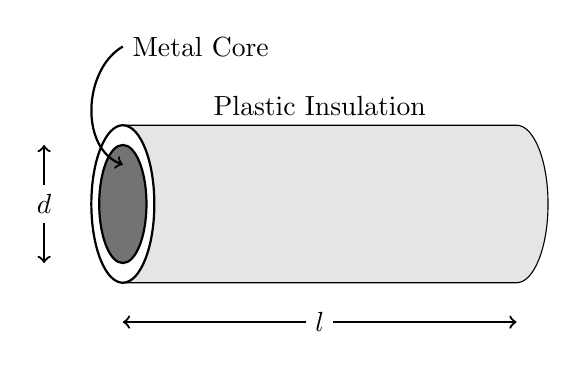
\begin{tikzpicture}
        %% Barrel
        \draw[fill=white!90!black] (0,1) -- (5,1) arc (90:-90:0.4cm and 1cm) -- (0,-1) arc(270:90:0.4cm and 1cm) --cycle;
        \draw[thick,fill=white] (0,0) circle (0.4cm and 1cm);
        \draw[thick,fill=white!45!black] (0,0) circle (0.3cm and 0.75cm);
        %% Labels
        \node[anchor=south] at (2.5,1) {Plastic Insulation};
        \node[anchor=west] (M) at (0,2) {Metal Core};
        \draw[thick,<-] (0,0.5) to[out=160,in=210] (M.west);
        %% Labels
        \draw[thick,<->] (0,-1.5) -- (5,-1.5) node[pos=0.5,anchor=center,fill=white] {$l$};
        \draw[thick,<->] (-1,0.75) -- (-1,-0.75) node[pos=0.5,anchor=center,fill=white] {$d$};
    \end{tikzpicture}
    \end{center}
    A decrease in the resistance of the wire would be produced by an increase in the:
    \begin{choices}
        \wrongchoice{thickness of the plastic insulation}
        \wrongchoice{length $l$ of the wire}
      \correctchoice{diameter $d$ of the wire}
        \wrongchoice{temperature of the wire}
    \end{choices}
\end{question}
}

\element{nysed}{
\begin{question}{June2001-Q29}
    Which diagram below correctly shows currents traveling near junction $P$ in an electric circuit?
    \begin{multicols}{2}
    \begin{choices}
        \AMCboxDimensions{down=-1.2cm}
        \ctikzset{bipoles/length=0.75cm}
        \wrongchoice{
            \begin{circuitikz}[yscale=0.8]
                \draw[white] (0,-1.5) -- (0,1.5);
                \draw[fill] (0,0) circle (1.5pt) node[anchor=west] {$P$};
                \draw (-2,0) to [short,i=\SI{3}{\ampere}] (0,0);
                \draw (0,0) to [short,i=\SI{4}{\ampere}] (0,2);
                \draw (0,-2) to [short,i=\SI{7}{\ampere}] (0,0);
            \end{circuitikz}
        }
        \wrongchoice{
            \begin{circuitikz}[yscale=0.8]
                \draw[white] (0,-1.5) -- (0,1.5);
                \draw[fill] (0,0) circle (1.5pt) node[anchor=west] {$P$};
                \draw (-2,0) to [short,i=\SI{3}{\ampere}] (0,0);
                \draw (0,2) to [short,i=\SI{4}{\ampere}] (0,0);
                \draw (0,-2) to [short,i=\SI{7}{\ampere}] (0,0);
            \end{circuitikz}
        }
        \wrongchoice{
            \begin{circuitikz}[yscale=0.8]
                \draw[white] (0,-1.5) -- (0,1.5);
                \draw[fill] (0,0) circle (1.5pt) node[anchor=west] {$P$};
                \draw (0,0) to [short,i=\SI{3}{\ampere}] (-2,0);
                \draw (0,2) to [short,i=\SI{4}{\ampere}] (0,0);
                \draw (0,-2) to [short,i=\SI{7}{\ampere}] (0,0);
            \end{circuitikz}
        }
        \correctchoice{
            \begin{circuitikz}[yscale=0.8]
                \draw[white] (0,-1.5) -- (0,1.5);
                \draw[fill] (0,0) circle (1.5pt) node[anchor=west] {$P$};
                \draw (0,0) to [short,i=\SI{3}{\ampere}] (-2,0);
                \draw (0,0) to [short,i=\SI{4}{\ampere}] (0,2);
                \draw (0,-2) to [short,i=\SI{7}{\ampere}] (0,0);
            \end{circuitikz}
        }
    \end{choices}
    \end{multicols}
\end{question}
}

\element{nysed}{
\begin{question}{June2001-Q30}
    The diagram below shows three resistors, $R_1$, $R_2$,
        and $R_3$, connected to a \SI{12}{\volt} battery.
    \begin{center}
    \ctikzset{bipoles/length=0.75cm}
    \begin{circuitikz}[xscale=1.5]
        %% NOTE: TODO: draw tikz, short,i
        \draw (0,0) to [battery,l=\SI{12}{\volt}] (0,2)
                    to [R,l_=$R_1$](2,2)
                    to [R,l_=$R_2$](2,0)
                    to [R,l=$R_3$](0,0);
        \draw (0.5,2) to (0.5,2.5)
                    to [voltmeter,l=$V_1$] (1.5,2.5)
                    to (1.5,2);
        \draw (2,1.5) to (2.5,1.5)
                    to [voltmeter,l=$V_2$] (2.5,0.5)
                    to (2,0.5);
    \end{circuitikz}
    \end{center}
    If voltmeter $V_1$ reads \SI{3}{\volt} and voltmeter $V_2$ reads \SI{4}{\volt},
        what is the potential drop across resistor $R_3$?
    \begin{multicols}{2}
    \begin{choices}
        \wrongchoice{\SI{12}{\volt}}
      \correctchoice{\SI{5}{\volt}}
        \wrongchoice{\SI{0}{\volt}}
        \wrongchoice{\SI{4}{\volt}}
    \end{choices}
    \end{multicols}
\end{question}
}

\element{nysed}{
\begin{question}{June2001-Q31}
    A current of \SI{3.0}{\ampere} is flowing in a circuit.
    How much charge passes a given point in the circuit in \SI{30}{\second}?
    \begin{multicols}{2}
    \begin{choices}
        \wrongchoice{\SI{0.10}{\coulomb}}
        \wrongchoice{\SI{10}{\coulomb}}
        \wrongchoice{\SI{33}{\coulomb}}
      \correctchoice{\SI{90}{\coulomb}}
    \end{choices}
    \end{multicols}
\end{question}
}

\newcommand{\myJuneZeroOneQthirtyTwoTikz}{
    \ctikzset{bipoles/length=0.75cm}
    \begin{circuitikz}[yscale=0.66]
        \draw (2,0)to [battery,l_=$\SI{6.0}{\volt}$] (-2,0)
                    to (-2,2)
                    to [R,l=$\SI{3.0}{\ohm}$] (2,2)
                    to (2,0);
        \draw (-2,2)to [ammeter,l=$A$] (-2,4)
                    to [R,l=$\SI{1.0}{\ohm}$] (2,4)
                    to (2,2);
    \end{circuitikz}
}

\element{nysed}{
\begin{question}{June2001-Q32}
    The diagram below shows two resistors connected in parallel across a \SI{6}{\volt} source.
    \begin{center}
        \myJuneZeroOneQthirtyTwoTikz
    \end{center}
    The equivalent resistance of the two resistors is:
    \begin{multicols}{2}
    \begin{choices}
      \correctchoice{\SI{0.75}{\ohm}}
        \wrongchoice{\SI{2.0}{\ohm}}
        \wrongchoice{\SI{1.3}{\ohm}}
        \wrongchoice{\SI{4.0}{\ohm}}
    \end{choices}
    \end{multicols}
\end{question}
}

\element{nysed}{
\begin{question}{June2001-Q33}
    The diagram below shows two resistors connected in parallel across a \SI{6}{\volt} source.
    \begin{center}
        \myJuneZeroOneQthirtyTwoTikz
    \end{center}
    Compared to the power dissipated in the \SI{1.0}{\ohm} resistor,
        the power dissipated in the \SI{3.0}{\ohm} resistor is:
    \begin{multicols}{2}
    \begin{choices}
      \correctchoice{less}
        \wrongchoice{greater}
        \wrongchoice{the same}
    \end{choices}
    \end{multicols}
\end{question}
}


%% Section Jan2001
%%--------------------
\element{nysed}{
\begin{question}{Jan2001-Q26}
    Compared to insulators, metals are better conductors of electricity because metals contain more free:
    \begin{multicols}{2}
    \begin{choices}
        \wrongchoice{protons}
      \correctchoice{electrons}
        \wrongchoice{positive ions}
        \wrongchoice{negative ions}
    \end{choices}
    \end{multicols}
\end{question}
}

\element{nysed}{
\begin{question}{Jan2001-Q27}
    If a \SI{15}{\ohm} resistor is connected in parallel with a \SI{30}{\ohm} resistor,
        the equivalent resistance is:
    \begin{multicols}{2}
    \begin{choices}
        \wrongchoice{\SI{15}{\ohm}}
        \wrongchoice{\SI{2.0}{\ohm}}
      \correctchoice{\SI{10}{\ohm}}
        \wrongchoice{\SI{45}{\ohm}}
    \end{choices}
    \end{multicols}
\end{question}
}

\element{nysed}{
\begin{question}{Jan2001-Q29}
    A metal wire has length $L$ and cross-sectional area $A$.
    The resistance of the wire is directly proportional to:
    \begin{multicols}{2}
    \begin{choices}
      \correctchoice{$\dfrac{L}{A}$}
        \wrongchoice{$L \times A$}
        \wrongchoice{$\dfrac{A}{L}$}
        \wrongchoice{$L + A$}
    \end{choices}
    \end{multicols}
\end{question}
}

\element{nysed}{
\begin{question}{Jan2001-Q30}
    The diagram below shows electric currents in conductors that meet at junction $P$.
    \begin{center}
    \begin{circuitikz}
        \draw[fill] (0,0) circle (2pt) node[anchor=north west] {$P$};
        \draw[fill] (2,0) circle (2pt) node[anchor=west] {$Q$};
        \draw (0,0) -- (2,0);
        \draw (-2,0) to [short,i=\SI{3}{\ampere}] (0,0);
        \draw (0,0) to [short,i=\SI{2}{\ampere}] (0,2);
        \draw (0,-2) to [short,i=\SI{4}{\ampere}] (0,0);
    \end{circuitikz}
    \end{center}
    What are the magnitude and direction of the current in conductor $PQ$?
    \begin{multicols}{2}
    \begin{choices}
        \wrongchoice{\SI{9}{\ampere} toward $P$}
        \wrongchoice{\SI{9}{\ampere} toward $Q$}
        \wrongchoice{\SI{5}{\ampere} toward $P$}
      \correctchoice{\SI{5}{\ampere} toward $Q$}
    \end{choices}
    \end{multicols}
\end{question}
}

%% completely reworded these questions
\newcommand{\myJanZeroOneQthirtyTwoTikz}{
    \ctikzset{bipoles/length=0.75cm}
    \begin{circuitikz}[xscale=1.40,font=\small]
        \draw (0,0) to [battery] (0,2)
                    to [ammeter,i^>=\SI{10}{\ampere}] (2,2)
                    to [R,l=\SI{6.0}{\ohm}](2,1)
                    to [ammeter,l=$A_1$] (2,0)
                    to (0,0);
        \draw (2,2) to (4,2)
                    to [R,l=$\SI{30}{\ohm}$] (4,1)
                    to [ammeter,i^>=\SI{4}{\ampere}] (4,0)
                    to (2,0);
    \end{circuitikz}
}

\element{nysed}{
\begin{question}{Jan2001-Q32}
    The diagram below shows two resistors and three ammeters connected to a voltage source.
    \begin{center}
        \myJanZeroOneQthirtyTwoTikz
    \end{center}
    What is the potential difference across the source?
    \begin{multicols}{2}
    \begin{choices}
        \wrongchoice{\SI{440}{\volt}}
        \wrongchoice{\SI{240}{\volt}}
      \correctchoice{\SI{120}{\volt}}
        \wrongchoice{\SI{60}{\volt}}
    \end{choices}
    \end{multicols}
\end{question}
}

\element{nysed}{
\begin{question}{Jan2001-Q33}
    The diagram below shows two resistors and three ammeters connected to a voltage source.
    \begin{center}
        \myJanZeroOneQthirtyTwoTikz
    \end{center}
    What is the current reading of ammeter $A_1$?
    \begin{multicols}{2}
    \begin{choices}
        \wrongchoice{\SI{10}{\ampere}}
      \correctchoice{\SI{6.0}{\ampere}}
        \wrongchoice{\SI{3.0}{\ampere}}
        \wrongchoice{\SI{4.0}{\ampere}}
    \end{choices}
    \end{multicols}
\end{question}
}

\element{nysed}{
\begin{question}{Jan2001-Q35}
    A wire carries a current of \SI{2.0}{\ampere}.
    How many electrons pass a given point in this wire in \SI{1.0}{\second}?
    \begin{multicols}{2}
    \begin{choices}
        \wrongchoice{\num{1.3e18}}
        \wrongchoice{\num{2.0e18}}
      \correctchoice{\num{1.3e19}}
        \wrongchoice{\num{2.0e19}}
    \end{choices}
    \end{multicols}
\end{question}
}

\element{nysed}{
\begin{question}{Jan2001-Q80}
    In order to measure the current through an electrical device,
        an ammeter is placed in series with the device.
    Compared to the electrical device,
        the ammeter should have a much:
    \begin{choices}
        \wrongchoice{lower permeability}
        \wrongchoice{higher permeability}
      \correctchoice{lower resistance}
        \wrongchoice{higher resistance}
    \end{choices}
\end{question}
}


%% Section June2000
%%--------------------
\element{nysed}{
\begin{question}{June2000-Q26}
    A lightning bolt transfers \SI{6.0}{\coulomb} of charge from a cloud to the ground in \SI{2.0e-3}{\second}.
    What is the average current during this event?
    \begin{multicols}{2}
    \begin{choices}
        \wrongchoice{\SI{1.2e-2}{\ampere}}
        \wrongchoice{\SI{3.0e2}{\ampere}}
      \correctchoice{\SI{3.0e3}{\ampere}}
        \wrongchoice{\SI{1.2e4}{\ampere}}
    \end{choices}
    \end{multicols}
\end{question}
}

\element{nysed}{
\begin{question}{June2000-Q27}
    Conductivity in metallic solids is due to the presence of free:
    \begin{multicols}{2}
    \begin{choices}
        \wrongchoice{nuclei}
        \wrongchoice{protons}
        \wrongchoice{neutrons}
      \correctchoice{electrons}
    \end{choices}
    \end{multicols}
\end{question}
}

\element{nysed}{
\begin{question}{June2000-Q32}
    The graph below represents the relationship between the potential difference across a metal conductor and the current through the conductor at a constant temperature.
    \begin{center}
    \begin{tikzpicture}
        \begin{axis}[
            axis y line=left,
            axis x line=bottom,
            axis line style={->},
            ylabel={potential},
            y unit=\si{\volt},
            ytick={0,2.0,4.0,6.0,8.0},
            xlabel={current},
            x unit=\si{\ampere},
            xtick={0,0.2,0.4,0.6,0.8},
            xmin=0,xmax=0.9,
            ymin=0,ymax=8,
            grid=major,
            width=0.8\columnwidth,
            height=0.5\columnwidth,
            very thin,
        ]
        \addplot[line width=1pt,domain=0:0.9]{10*x};
        \end{axis}
    \end{tikzpicture}
    \end{center}
    What is the resistance of the conductor?
    \begin{multicols}{2}
    \begin{choices}
        \wrongchoice{\SI{1}{\ohm}}
        \wrongchoice{\SI{0.01}{\ohm}}
        \wrongchoice{\SI{0.1}{\ohm}}
      \correctchoice{\SI{10}{\ohm}}
    \end{choices}
    \end{multicols}
\end{question}
}

\element{nysed}{
\begin{question}{June2000-Q35}
    The diagram below shows two resistors connected in series to a \SI{20}{\volt} battery.
    \begin{center}
    \ctikzset{bipoles/length=0.75cm}
    \begin{circuitikz}
        \draw (0,0) to [battery,l=\SI{20}{\volt}] (0,2)
                    to [R,l=\SI{5.0}{\ohm}] (2,2)
                    to [R,l=\SI{15.0}{\ohm}] (2,0)
                    to (0,0);
    \end{circuitikz}
    \end{center}
    If the current through the \SI{5.0}{\ohm} resistor is \SI{1.0}{\ampere},
        then current through the \SI{15}{\ohm} resistor is:
    \begin{multicols}{2}
    \begin{choices}
      \correctchoice{\SI{1.0}{\ampere}}
        \wrongchoice{\SI{0.33}{\ampere}}
        \wrongchoice{\SI{3.0}{\ampere}}
        \wrongchoice{\SI{1.3}{\ampere}}
    \end{choices}
    \end{multicols}
\end{question}
}

\element{nysed}{
\begin{question}{June2000-Q36}
    Resistors $R_1$ and $R_2$ have an equivalent resistance of \SI{6}{\ohm} when connected in the circuit shown below.
    \begin{center}
    \ctikzset{bipoles/length=0.75cm}
    \begin{circuitikz}
        \draw (0,0) to [battery] (0,2)
                    to (2,2)
                    to [R,l=$R_1$] (2,0)
                    to (0,0);
        \draw (2,2) to (4,2)
                    to [R,l=$R_2$] (4,0)
                    to (2,0);
    \end{circuitikz}
    \end{center}
    The resistance of $R_1$ could be:
    \begin{multicols}{2}
    \begin{choices}
        \wrongchoice{\SI{1}{\ohm}}
        \wrongchoice{\SI{5}{\ohm}}
      \correctchoice{\SI{8}{\ohm}}
        \wrongchoice{\SI{4}{\ohm}}
    \end{choices}
    \end{multicols}
\end{question}
}

\element{nysed}{
\begin{question}{June2000-Q37}
    The diagram below represents an electric circuit.
    \begin{center}
    \ctikzset{bipoles/length=0.75cm}
    \begin{circuitikz}
        \draw (0,0) to [battery] (0,2)
                    to (2,2)
                    to [R,l_=\SI{8}{\ohm}] (2,0)
                    to (0,0);
        \draw (2,1.5) to (3,1.5)
                    to [voltmeter,l=\SI{4}{\volt}] (3,0.5)
                    to (2,0.5);
    \end{circuitikz}
    \end{center}
    The total amount of energy delivered to the resistor in \SI{10}{\second} is:
    \begin{multicols}{2}
    \begin{choices}
        \wrongchoice{\SI{3.2}{\joule}}
        \wrongchoice{\SI{5.0}{\joule}}
      \correctchoice{\SI{20}{\joule}}
        \wrongchoice{\SI{320}{\joule}}
    \end{choices}
    \end{multicols}
\end{question}
}

\element{nysed}{
\begin{question}{June2000-Q39}
    A copper wire is part of a complete circuit through which current flows.
    Which graph best represents the relationship between the wire's length and its resistance?
    \begin{multicols}{2}
    \begin{choices}
        \AMCboxDimensions{down=-2.5em}
        \correctchoice{
            \begin{tikzpicture}
                \begin{axis}[
                    axis y line=left,
                    axis x line=bottom,
                    axis line style={->},
                    ylabel={length},
                    ytick=\empty,
                    xlabel={resistance},
                    xtick=\empty,
                    xmin=0,xmax=11,
                    ymin=0,ymax=11,
                    width=\columnwidth,
                    very thin,
                ]
                \addplot[line width=1pt,domain=0:10]{x};
                \end{axis}
            \end{tikzpicture}
        }
        \wrongchoice{
            \begin{tikzpicture}
                \begin{axis}[
                    axis y line=left,
                    axis x line=bottom,
                    axis line style={->},
                    ylabel={length},
                    ytick=\empty,
                    xlabel={resistance},
                    xtick=\empty,
                    xmin=0,xmax=11,
                    ymin=0,ymax=11,
                    width=\columnwidth,
                    very thin,
                ]
                \addplot[line width=1pt,domain=0:10]{5};
                \end{axis}
            \end{tikzpicture}
        }
        \wrongchoice{
            \begin{tikzpicture}
                \begin{axis}[
                    axis y line=left,
                    axis x line=bottom,
                    axis line style={->},
                    ylabel={length},
                    ytick=\empty,
                    xlabel={resistance},
                    xtick=\empty,
                    xmin=0,xmax=11,
                    ymin=0,ymax=11,
                    width=\columnwidth,
                    very thin,
                ]
                \addplot[line width=1pt,domain=0:10]{10-x};
                \end{axis}
            \end{tikzpicture}
        }
        \wrongchoice{
            \begin{tikzpicture}
                \begin{axis}[
                    axis y line=left,
                    axis x line=bottom,
                    axis line style={->},
                    ylabel={length},
                    ytick=\empty,
                    xlabel={resistance},
                    xtick=\empty,
                    xmin=0,xmax=11,
                    ymin=0,ymax=11,
                    width=\columnwidth,
                    very thin,
                ]
                \addplot[line width=1pt,domain=0:10]{10/x};
                \end{axis}
            \end{tikzpicture}
        }
    \end{choices}
    \end{multicols}
\end{question}
}


\element{nysed}{
\begin{question}{June2000-Q40}
    The heating element on an electric stove dissipates \SI{4.0e2}{\watt} of power when connected to a \SI{120}{\volt} source.
    What is the electrical resistance of this heating element?
    \begin{multicols}{2}
    \begin{choices}
        \wrongchoice{\SI{0.028}{\ohm}}
        \wrongchoice{\SI{0.60}{\ohm}}
        \wrongchoice{\SI{3.3}{\ohm}}
      \correctchoice{\SI{36}{\ohm}}
    \end{choices}
    \end{multicols}
\end{question}
}

\element{nysed}{
\begin{question}{June2000-Q77}
    A simple electrical circuit contains a battery,
        a light bulb, and a properly connected ammeter.
    The ammeter has a very low internal resistance because it is connect in:
    \begin{choices}
        \wrongchoice{parallel with the bulb to have little effect on the current through the bulb}
        \wrongchoice{parallel with the bulb to prevent current flow through the bulb}
      \correctchoice{series with the bulb to have little effect on the current through the bulb}
        \wrongchoice{series with the bulb to prevent current flow through the bulb}
    \end{choices}
\end{question}
}


%% Section June1999
%%--------------------
\element{nysed}{
\begin{question}{June1999-Q31}
    A metallic conductor obeys Ohm's law.
    Which graph best represents the relationship between the potential difference across the conductor and the resulting current through the conductor?
    \begin{multicols}{2}
    \begin{choices}
        \AMCboxDimensions{down=-2.5em}
        \correctchoice{
            \begin{tikzpicture}
                \begin{axis}[
                    axis y line=left,
                    axis x line=bottom,
                    axis line style={->},
                    ylabel={potential},
                    ytick=\empty,
                    xlabel={current},
                    xtick=\empty,
                    xmin=0,xmax=11,
                    ymin=0,ymax=11,
                    width=\columnwidth,
                    very thin,
                ]
                \addplot[line width=1pt,domain=0:10]{x};
                \end{axis}
            \end{tikzpicture}
        }
        \wrongchoice{
            \begin{tikzpicture}
                \begin{axis}[
                    axis y line=left,
                    axis x line=bottom,
                    axis line style={->},
                    ylabel={potential},
                    ytick=\empty,
                    xlabel={current},
                    xtick=\empty,
                    xmin=0,xmax=11,
                    ymin=0,ymax=11,
                    width=\columnwidth,
                    very thin,
                ]
                \addplot[line width=1pt,domain=0:10]{5};
                \end{axis}
            \end{tikzpicture}
        }
        \wrongchoice{
            \begin{tikzpicture}
                \begin{axis}[
                    axis y line=left,
                    axis x line=bottom,
                    axis line style={->},
                    ylabel={potential},
                    ytick=\empty,
                    xlabel={current},
                    xtick=\empty,
                    xmin=0,xmax=11,
                    ymin=0,ymax=11,
                    width=\columnwidth,
                    very thin,
                ]
                \addplot[line width=1pt,domain=0:10]{10-x};
                \end{axis}
            \end{tikzpicture}
        }
        \wrongchoice{
            \begin{tikzpicture}
                \begin{axis}[
                    axis y line=left,
                    axis x line=bottom,
                    axis line style={->},
                    ylabel={potential},
                    ytick=\empty,
                    xlabel={current},
                    xtick=\empty,
                    xmin=0,xmax=11,
                    ymin=0,ymax=11,
                    width=\columnwidth,
                    very thin,
                ]
                \addplot[line width=1pt,domain=0:10]{10/x};
                \end{axis}
            \end{tikzpicture}
        }
    \end{choices}
    \end{multicols}
\end{question}
}

\element{nysed}{
\begin{question}{June1999-Q32}
    A light bulb operating at \SI{120}{\volt} draws a current of \SI{0.50}{\ampere} for \SI{240}{\second}.
    The power rating of the light bulb is:
    \begin{multicols}{2}
    \begin{choices}
        \wrongchoice{\SI{30}{\watt}}
      \correctchoice{\SI{60}{\watt}}
        \wrongchoice{\SI{75}{\watt}}
        \wrongchoice{\SI{120}{\watt}}
    \end{choices}
    \end{multicols}
\end{question}
}

\element{nysed}{
\begin{question}{June1999-Q33}
    In the diagram below of a parallel circuit,
        ammeter $A$ measures the current supplied by the \SI{110}{\volt} source.
    \begin{center}
    \ctikzset{bipoles/length=0.75cm}
    \begin{circuitikz}[xscale=1.75]
        \draw (0,0) to [battery,l=\SI{110}{\volt}] (0,2)
                    to (3,2) 
                    to (3,1) to [R,l_=\SI{60}{\ohm}] (3,0)
                    to (1,0) to [ammeter,l_=$A$] (0,0);
        \draw (2,2) to [R,l_=\SI{30}{\ohm}] (2,0);
        \draw (1,2) to [R,l_=\SI{20}{\ohm}] (1,1) to (1,0);
    \end{circuitikz}
    \end{center}
    The current measured by ammeter $A$ is:
    \begin{multicols}{2}
    \begin{choices}
        \wrongchoice{\SI{1.0}{\ampere}}
        \wrongchoice{\SI{0.10}{\ampere}}
        \wrongchoice{\SI{5.5}{\ampere}}
      \correctchoice{\SI{11}{\ampere}}
    \end{choices}
    \end{multicols}
\end{question}
}

\element{nysed}{
\begin{question}{June1999-Q35}
    The diagram below represents a simple electric circuit.
    \begin{center}
    \ctikzset{bipoles/length=0.75cm}
    \begin{circuitikz}[xscale=1.75,yscale=0.9]
        \draw (0,0) to [battery,l=\SI{12}{\volt}] (0,2)
                    to [R,l=\SI{3.0}{\ohm}] (2,2)
                    to (2,0)
                    to [ammeter,i>=\SI{4.0}{\ampere}] (0,0);
    \end{circuitikz}
    \end{center}
    How much charge passes through the resistor in \SI{2.0}{\second}?
    \begin{multicols}{2}
    \begin{choices}
        \wrongchoice{\SI{6.0}{\coulomb}}
        \wrongchoice{\SI{2.0}{\coulomb}}
      \correctchoice{\SI{8.0}{\coulomb}}
        \wrongchoice{\SI{4.0}{\coulomb}}
    \end{choices}
    \end{multicols}
\end{question}
}

\element{nysed}{
\begin{question}{June1999-Q37}
    The table below shows the length and cross-sectional area of four pieces of copper wire at the same temperature.
    \begin{center}
    \begin{tabu}{ccc}
        \multicolumn{1}{l}{Wire} & 
        \multicolumn{1}{l}{Length (\si{\meter})} &
        \multicolumn{1}{l}{Cross-Sectional Area (\si{\meter\squared})} \\
        \midrule
        $I$ & 10 & \num{2e-6} \\
        $J$ & 10 & \num{1e-6} \\
        $K$ & 1  & \num{2e-6} \\
        $L$ & 1  & \num{1e-6} \\
    \end{tabu}
    \end{center}
    Which wire has the highest resistance?
    \begin{multicols}{4}
    \begin{choices}
        \wrongchoice{$I$}
      \correctchoice{$J$}
        \wrongchoice{$K$}
        \wrongchoice{$L$}
    \end{choices}
    \end{multicols}
\end{question}
}

\element{nysed}{
\begin{question}{June1999-Q76}
    Which graph best represents the relationship between the deflection of a galvonometer coil and the current passing through the coil?
    \begin{multicols}{2}
    \begin{choices}
        \AMCboxDimensions{down=-2.5em}
        \correctchoice{
            \begin{tikzpicture}
                \begin{axis}[
                    axis y line=left,
                    axis x line=bottom,
                    axis line style={->},
                    ylabel={deflection},
                    ytick=\empty,
                    xlabel={current},
                    xtick=\empty,
                    xmin=0,xmax=11,
                    ymin=0,ymax=11,
                    width=\columnwidth,
                    very thin,
                ]
                \addplot[line width=1pt,domain=0:10]{x};
                \end{axis}
            \end{tikzpicture}
        }
        \wrongchoice{
            \begin{tikzpicture}
                \begin{axis}[
                    axis y line=left,
                    axis x line=bottom,
                    axis line style={->},
                    ylabel={deflection},
                    ytick=\empty,
                    xlabel={current},
                    xtick=\empty,
                    xmin=0,xmax=11,
                    ymin=0,ymax=11,
                    width=\columnwidth,
                    very thin,
                ]
                \addplot[line width=1pt,domain=0:10]{0.1*x^2};
                \end{axis}
            \end{tikzpicture}
        }
        \wrongchoice{
            \begin{tikzpicture}
                \begin{axis}[
                    axis y line=left,
                    axis x line=bottom,
                    axis line style={->},
                    ylabel={deflection},
                    ytick=\empty,
                    xlabel={current},
                    xtick=\empty,
                    xmin=0,xmax=11,
                    ymin=0,ymax=11,
                    width=\columnwidth,
                    very thin,
                ]
                \addplot[line width=1pt,domain=0:10]{10/x};
                \end{axis}
            \end{tikzpicture}
        }
        \wrongchoice{
            \begin{tikzpicture}
                \begin{axis}[
                    axis y line=left,
                    axis x line=bottom,
                    axis line style={->},
                    ylabel={deflection},
                    ytick=\empty,
                    xlabel={current},
                    xtick=\empty,
                    xmin=0,xmax=11,
                    ymin=0,ymax=11,
                    width=\columnwidth,
                    very thin,
                ]
                \addplot[line width=1pt,domain=0:10]{8};
                \end{axis}
            \end{tikzpicture}
        }
    \end{choices}
    \end{multicols}
\end{question}
}


%% Section June1998
%%--------------------
\element{nysed}{
\begin{question}{June1998-Q27}
    What is the potential difference across a \SI{2.0}{\ohm} resistor that draws \SI{2.0}{\coulomb\per\second}?
    \begin{multicols}{2}
    \begin{choices}
        \wrongchoice{\SI{1.0}{\volt}}
        \wrongchoice{\SI{2.0}{\volt}}
        \wrongchoice{\SI{3.0}{\volt}}
      \correctchoice{\SI{4.0}{\volt}}
    \end{choices}
    \end{multicols}
\end{question}
}

\element{nysed}{
\begin{question}{June1998-Q28}
    The diagram below shows a circuit with three resistors.
    \begin{center}
    \ctikzset{bipoles/length=0.75cm}
    \begin{circuitikz}[xscale=1.50]
        \draw (0,0) to [battery,l=\SI{24}{\volt}] (1,0)
                    to [ammeter,i>=\SI{2.0}{\ampere}] (3,0)
                    to (3,2)
                    to [R,l=$R$] (2,2)
                    to [R,l=\SI{6.0}{\ohm}] (1,2)
                    to [R,l=\SI{4.0}{\ohm}] (0,2)
                    to (0,0);
    \end{circuitikz}
    \end{center}
    What is the resistance of resistor $R$?
    \begin{multicols}{2}
    \begin{choices}
        \wrongchoice{\SI{6.0}{\ohm}}
      \correctchoice{\SI{2.0}{\ohm}}
        \wrongchoice{\SI{12}{\ohm}}
        \wrongchoice{\SI{4.0}{\ohm}}
    \end{choices}
    \end{multicols}
\end{question}
}

\element{nysed}{
\begin{question}{June1998-Q29}
    Three ammeters are placed in a circuit as shown below.
    \begin{center}
    \ctikzset{bipoles/length=0.75cm}
    \begin{circuitikz}[xscale=1.33]
        \draw (0,0) to [battery] (0,2)
                    to [ammeter,l_=$A_1$] (2,2)
                    to [ammeter,l=$A_2$] (2,1)
                    to [R] (2,0)
                    to (0,0);
        \draw (2,2) to (4,2)
                    to [ammeter,l=$A_3$] (4,1)
                    to [R] (4,0)
                    to (2,0);
    \end{circuitikz}
    \end{center}
    If $A_1$ reads \SI{5}{\ampere} and $A_2$ reads \SI{2.0}{\ampere},
        what does $A_3$ read?
    \begin{multicols}{2}
    \begin{choices}
        \wrongchoice{\SI{1.0}{\ampere}}
        \wrongchoice{\SI{2.0}{\ampere}}
      \correctchoice{\SI{3.0}{\ampere}}
        \wrongchoice{\SI{7.0}{\ampere}}
    \end{choices}
    \end{multicols}
\end{question}
}

\element{nysed}{
\begin{question}{June1998-Q30}
    An electric motor draws \SI{150}{\ampere} of current while operating at \SI{240}{\volt}.
    What is the power rating of this motor?
    \begin{multicols}{2}
    \begin{choices}
        \wrongchoice{\SI{1.6}{\watt}}
        \wrongchoice{\SI{3.8e2}{\watt}}
      \correctchoice{\SI{3.6e4}{\watt}}
        \wrongchoice{\SI{5.4e6}{\watt}}
    \end{choices}
    \end{multicols}
\end{question}
}

\element{nysed}{
\begin{question}{June1998-Q31}
    An operating \SI{75}{\watt} lamp is connected to a \SI{120}{\volt} outlet.
    How much electrical energy is used by the lamp in \SI{60}{\minute} (\SI{3600}{\second})?
    \begin{multicols}{2}
    \begin{choices}
        \wrongchoice{\SI{4.5e3}{\joule}}
      \correctchoice{\SI{2.7e5}{\joule}}
        \wrongchoice{\SI{5.4e5}{\joule}}
        \wrongchoice{\SI{3.2e7}{\joule}}
    \end{choices}
    \end{multicols}
\end{question}
}

%%% NOTE: TOOD: Q32 requires graphics
%\element{nysed}{
%\begin{question}{June1998-Q32}
%    In which pair of circuits shown below could the readins
%        of voltmeters $V_1$ and $V_2$ and ammeter $A$ be correct?
%    \begin{multicols}{2}
%    \begin{choices}
%        \AMCboxDimensions{down=-2.5em}
%        \correctchoice{
%            \ctikzset{bipoles/length=0.75cm}
%            \begin{circuitikz}[scale=1.0]
%                \draw (0,0) to [battery] (0,2)
%                            to (2,2)
%                            to [R,l_=$R_2$] (2,0)
%                            to [ospst=$S$,mirror] (1,0)
%                            to (0,0);
%                \draw (1,2) to [R,l_=$R_1$] (1,0);
%            \end{circuitikz}
%        }
%        \wrongchoice{
%            \ctikzset{bipoles/length=0.75cm}
%            \begin{circuitikz}[scale=1.0]
%                \draw (0,0) to [battery] (0,2)
%                            to [R,l_=$R_1$] (2,2)
%                            to [ospst=$S$,mirror] (2,0)
%                            to [R,l_=$R_2$] (0,0);
%            \end{circuitikz}
%        }
%        \wrongchoice{
%            \ctikzset{bipoles/length=0.75cm}
%            \begin{circuitikz}[scale=1.0]
%                \draw (0,0) to [battery] (0,2)
%                            to (2,2)
%                            to [R,l_=$R_2$] (2,0)
%                            to (1,0)
%                            to [ospst=$S$,mirror] (0,0);
%                \draw (1,2) to [R,l_=$R_1$] (1,0);
%            \end{circuitikz}
%        }
%        \wrongchoice{
%            \ctikzset{bipoles/length=0.75cm}
%            \begin{circuitikz}[scale=1.0]
%                \draw (0,0) to [battery] (0,2)
%                            to (2,2)
%                            to [R,l_=$R_2$] (2,0)
%                            to (0,0);
%                \draw (1,2) to [R,l_=$R_1$] (1,1)
%                            to [ospst=$S$,mirror] (1,0);
%            \end{circuitikz}
%        }
%    \end{choices}
%    \end{multicols}
%\end{question}
%}

\element{nysed}{
\begin{question}{June1998-Q53}
    When an incandescent light bulb is turned on,
        its thin wire filament heats up quickly.
    As the temperature of this wire filament increases,
        its electrical resistance:
    \begin{choices}
        \wrongchoice{decreases}
      \correctchoice{increases}
        \wrongchoice{remains the same}
    \end{choices}
\end{question}
}

\element{nysed}{
\begin{question}{June1998-Q79}
    Which device consists of a galvanometer with a low-resistance shunt placed in parallel across its terminals?
    \begin{choices}
        \wrongchoice{mass spectrometer}
        \wrongchoice{transformer}
      \correctchoice{voltmeter}
        \wrongchoice{ammeter}
    \end{choices}
\end{question}
}


%% Section June1997
%%--------------------
\element{nysed}{
\begin{question}{June1997-Q27}
    The diagram below shows currents in a segment of an electric circuit.
    \begin{center}
    \ctikzset{bipoles/length=0.75cm}
    \begin{circuitikz}[scale=0.8]
        \draw[thick] (3,0) to [short,i^>=\SI{2}{\ampere}] (0,0)
                           to [short,i^>=\SI{5}{\ampere}] (-3,0);
        \draw[thick] (0,2) to [short,i^>=\SI{6}{\ampere}] (0,0)
                           to [ammeter,l=$A$] (0,-2);
    \end{circuitikz}
    \end{center}
    What is the reading on ammeter $A$?
    \begin{multicols}{2}
    \begin{choices}
        \wrongchoice{\SI{8}{\ampere}}
        \wrongchoice{\SI{2}{\ampere}}
      \correctchoice{\SI{3}{\ampere}}
        \wrongchoice{\SI{13}{\ampere}}
    \end{choices}
    \end{multicols}
\end{question}
}

\element{nysed}{
\begin{question}{June1997-Q28}
    An operating lamp draws a current of \SI{0.5}{\ampere}.
    The amount of charge passing through the lamp in \SI{10}{\second} is:
    \begin{multicols}{2}
    \begin{choices}
        \wrongchoice{\SI{0.050}{\coulomb}}
        \wrongchoice{\SI{2.0}{\coulomb}}
      \correctchoice{\SI{5.0}{\coulomb}}
        \wrongchoice{\SI{20}{\coulomb}}
    \end{choices}
    \end{multicols}
\end{question}
}

\element{nysed}{
\begin{question}{June1997-Q29}
    Which graph best represents the relationship between the resistance of a copper wire of uniform cross-sectional area and the wire's length at constant temperature?
    \begin{multicols}{2}
    \begin{choices}
        \AMCboxDimensions{down=-2.5em}
        \correctchoice{
            \begin{tikzpicture}
                \begin{axis}[
                    axis y line=left,
                    axis x line=bottom,
                    axis line style={->},
                    ylabel={resistance},
                    ytick=\empty,
                    xlabel={length},
                    xtick=\empty,
                    xmin=0,xmax=11,
                    ymin=0,ymax=11,
                    width=\columnwidth,
                    very thin,
                ]
                \addplot[line width=1pt,domain=0:10]{x};
                \end{axis}
            \end{tikzpicture}
        }
        \wrongchoice{
            \begin{tikzpicture}
                \begin{axis}[
                    axis y line=left,
                    axis x line=bottom,
                    axis line style={->},
                    ylabel={resistance},
                    ytick=\empty,
                    xlabel={length},
                    xtick=\empty,
                    xmin=0,xmax=11,
                    ymin=0,ymax=11,
                    width=\columnwidth,
                    very thin,
                ]
                \addplot[line width=1pt,domain=0:10]{5};
                \end{axis}
            \end{tikzpicture}
        }
        \wrongchoice{
            \begin{tikzpicture}
                \begin{axis}[
                    axis y line=left,
                    axis x line=bottom,
                    axis line style={->},
                    ylabel={resistance},
                    ytick=\empty,
                    xlabel={length},
                    xtick=\empty,
                    xmin=0,xmax=11,
                    ymin=0,ymax=11,
                    width=\columnwidth,
                    very thin,
                ]
                \addplot[line width=1pt,domain=0:10]{10-x};
                \end{axis}
            \end{tikzpicture}
        }
        \wrongchoice{
            \begin{tikzpicture}
                \begin{axis}[
                    axis y line=left,
                    axis x line=bottom,
                    axis line style={->},
                    ylabel={resistance},
                    ytick=\empty,
                    xlabel={length},
                    xtick=\empty,
                    xmin=0,xmax=11,
                    ymin=0,ymax=11,
                    width=\columnwidth,
                    very thin,
                ]
                \addplot[line width=1pt,domain=0:10]{10/x};
                \end{axis}
            \end{tikzpicture}
        }
    \end{choices}
    \end{multicols}
\end{question}
}


\element{nysed}{
\begin{question}{June1997-Q31}
    To increase the brightness of a desk lamp,
        a student replaces a \SI{60}{\watt} light bulb with a \SI{100}{\watt} light bulb.
    Compared to the \SI{60}{\watt} bulb,
        the \SI{100}{\watt} bulb has:
    \begin{choices}
      \correctchoice{less resistance and draws more current.}
        \wrongchoice{less resistance and draws less current.}
        \wrongchoice{more resistance and draws more current.}
        \wrongchoice{more resistance and draws less current.}
    \end{choices}
\end{question}
}

\element{nysed}{
\begin{question}{June1997-Q32}
    An electric dryer consumed \SI{6.0e6}{\joule} of energy when operating at \SI{220}{\volt} for \SI{30}{\minute} (\SI{1800}{\second}).
    During operation, the dryer draws a current of approximately:
    \begin{multicols}{2}
    \begin{choices}
        \wrongchoice{\SI{10}{\ampere}}
      \correctchoice{\SI{15}{\ampere}}
        \wrongchoice{\SI{20}{\ampere}}
        \wrongchoice{\SI{25}{\ampere}}
    \end{choices}
    \end{multicols}
\end{question}
}


%% Section June1996
%%--------------------
\element{nysed}{
\begin{question}{June1996-Q29}
    A metal conductor is used in an electric circuit.
    The electrical resistance provided by the conductor could be increase by:
    \begin{choices}
        \wrongchoice{decreasing the length of the conductor.}
        \wrongchoice{decreasing the applied voltage in the circuit.}
      \correctchoice{increasing the temperature of the conductor.}
        \wrongchoice{increasing the cross-sectional area of the conductor.}
    \end{choices}
\end{question}
}

\element{nysed}{
\begin{question}{June1996-Q30}
    In the circuit shown below, voltmeter $V_2$ reads \SI{80}{\volt}.
    \begin{center}
    \begin{circuitikz}
        %% NOTE: TODO: circuitikz
    \end{circuitikz}
    \end{center}
    What is the reading of voltmeter $V_1$?
    \begin{multicols}{2}
    \begin{choices}
      \correctchoice{\SI{160}{\volt}}
        \wrongchoice{\SI{80}{\volt}}
        \wrongchoice{\SI{40}{\volt}}
        \wrongchoice{\SI{20}{\volt}}
    \end{choices}
    \end{multicols}
\end{question}
}

\element{nysed}{
\begin{question}{June1996-Q31}
    In a lightning strike,
        a charge of \SI{18}{\coulomb} is transferred between a cloud and the ground in \SI{2.0e-2}{\second} at a potential difference of \SI{1.5e6}{\volt}.
    What is the average current produced by this strike?
    \begin{multicols}{2}
    \begin{choices}
        \wrongchoice{\SI{3.6e-1}{\ampere}}
      \correctchoice{\SI{9.0e2}{\ampere}}
        \wrongchoice{\SI{3.0e4}{\ampere}}
        \wrongchoice{\SI{7.5e7}{\ampere}}
    \end{choices}
    \end{multicols}
\end{question}
}

\element{nysed}{
\begin{question}{June1996-Q32}
    The diagram below shows the current in a segment of a direct current circuit.
    \begin{center}
    \ctikzset{bipoles/length=0.75cm}
    \begin{circuitikz}[scale=0.8]
        \draw[thick] (-3,0) to [short,i^>=\SI{4}{\ampere}] (0,0)
                            to [short,i^>=\SI{8}{\ampere}] (3,0);
        \draw[thick] (0,2)  to [short,i^>=\SI{3}{\ampere}] (0,0)
                            to [ammeter,l=$A$] (0,-2);
    \end{circuitikz}
    \end{center}
    What is the reading of ammeter $A$?
    \begin{multicols}{2}
    \begin{choices}
        \wrongchoice{\SI{1}{\ampere}}
      \correctchoice{\SI{5}{\ampere}}
        \wrongchoice{\SI{7}{\ampere}}
        \wrongchoice{\SI{8}{\ampere}}
    \end{choices}
    \end{multicols}
\end{question}
}

\element{nysed}{
\begin{question}{June1996-Q36}
    If the potential drop across an operating \SI{300}{\watt} flood-light is \SI{120}{\volt},
        what is the current through the floodlight?
    \begin{multicols}{2}
    \begin{choices}
        \wrongchoice{\SI{0.40}{\ampere}}
      \correctchoice{\SI{2.5}{\ampere}}
        \wrongchoice{\SI{7.5}{\ampere}}
        \wrongchoice{\SI{4.8}{\ampere}}
    \end{choices}
    \end{multicols}
\end{question}
}

\endinput


